                                                                   % RSS 2016 High Level Control of Modular Robots
%%%%%%%%%%%%%%%%%%%%%%%%%%%%%%%%%%%%%%%%%%%%%%%%%%%%%%%%%%%%%%%%%
%%%                    Included packages                 %%%
%%%%%%%%%%%%%%%%%%%%%%%%%%%%%%%%%%%%%%%%%%%%%%%%%%%%%%%%%%%%%%%%%

%%%  Included by IEEE:

\documentclass[conference]{IEEEtran}
\usepackage{times}

% numbers option provides compact numerical references in the text. 
\usepackage[numbers]{natbib}
\usepackage{multicol}
\usepackage[bookmarks=true]{hyperref}

%%%%%%%%%%%%%%%%%%%%%%%%%%%%%%%%%%%%%%%%%%%%%%%%%%%%%%%%%%%%%%%%%
%%%   Additional packages:

\usepackage{pdfsync}
\usepackage[dvipsnames,table]{xcolor}
\usepackage{mathtools}
\usepackage{amsmath} % assumes amsmath package installed
\usepackage{amssymb}  % assumes amsmath package installed
%\usepackage[final]{pdfpages} % for including pdfs
\usepackage{subcaption}
\usepackage{multirow}
\usepackage{float}
\usepackage{amsmath}
\usepackage{nccmath} % for fleqn
\usepackage{algorithm}

%%%%%%%%%%%%%%%%%%%%%%%%%%%%%%%%%%%%%%%%%%%%%%%%%%%%%%%%%%%%%%%%%
%%%  Macros:

\newcommand{\separator}{ \noindent \rule{\columnwidth}{1pt} }
\newenvironment{old}{\color{Maroon} \separator \textbf{[\textit{Old:}]} }{\ignorespacesafterend \separator}
\newenvironment{new}{\color{Blue} \separator \textbf{[\textit{New:}]} }{\ignorespacesafterend \separator}
\newenvironment{notes}{\color{Gray} \separator}{\ignorespacesafterend \separator}

% For making things invisible during double-blind review. Put "#1" in the
% the braces to make the text appear later.:
\newcommand{\doubleBlind}[1]{} 

% For marking Todos and changes
\newcommand{\TODO}[1]{ {\bf \textcolor{red}{TODO:} #1 }}
\newcommand{\abj}[1]{\textcolor{blue}{#1}}
\newcommand{\dbj}[1]{\textcolor{blue}{\sout{#1}}}
\newcommand{\cbj}[2]{\textcolor{blue}{\sout{#1}}\textcolor{blue}{~#2}}
%\newcommand{\abt}[1]{\textcolor{magenta}{#1}}
% Handy commands
\newcommand{\lt}{{\tt True }}
\newcommand{\lf}{{\tt False }}
\newcommand{\ltnsp}{{\tt True}}
\newcommand{\lfnsp}{{\tt False}}
\newtheorem{definition}{Definition}
\DeclareMathOperator{\F}{\rotatebox[origin=c]{45}{$\Box$}}
\DeclareMathOperator{\X}{\bigcirc}
\DeclareMathOperator{\G}{\Box}
\newcommand{\LTLG}{\G}
\newcommand{\LTLF}{\F}
\newcommand{\LTLX}{\X}

\newfloat{spec}{thb}{lop} %{thb}{lop}
\floatname{spec}{Specification}
\makeatletter
\newcommand{\leqnomode}{\tagsleft@true}
\newcommand{\reqnomode}{\tagsleft@false}
\makeatother
%%%%%%%%%%%%%%%%%%%%%%%%%%%%%%%%%%%%%%%%%%%%%%%%%%%%%%%%%%%%%%%%%

\pdfinfo{
   /Author (Mystery Authors)
   /Title  () %TODO add title
   /CreationDate ()
   /Subject ()
   /Keywords ()
}

%%%%%%%%%%%%%%%%%%%%%%%%%%%%%%%%%%%%%%%%%%%%%%%%%%%%%%%%%%%%%%%%
%%%                     Main document                        %%%
%%%%%%%%%%%%%%%%%%%%%%%%%%%%%%%%%%%%%%%%%%%%%%%%%%%%%%%%%%%%%%%%
\usepackage{graphicx}

\begin{document}


\title{An Integrated System for Perception-Driven Autonomy with Modular Robots}

%\author{Mystery Authors}

\author{\authorblockN{Gangyuan Jing}
\authorblockA{
Cornell University\\
\texttt{gj56@cornell.edu}}
\and
\authorblockN{Tarik Tosun}
\authorblockA{Univ. of Pennsylvania\\
\texttt{tarikt@grasp.upenn.edu}}
\and
\authorblockN{Mark Yim}
\authorblockA{Univ. of Pennsylvania\\
\texttt{yim@grasp.upenn.edu}}
\and
\authorblockN{Hadas Kress-Gazit}
\authorblockA{Cornell University\\
\texttt{hadaskg@cornell.edu}}
}

\maketitle

\begin{abstract}

We present an integrated system that allows self-reconfigurable modular robots to autonomously accomplish perception-informed high-level tasks in an unknown environment, without any external sensing or control.  By performing three hardware experiments, we demonstrate that our system is capable of autonomously completing different object manipulation tasks in different environments without human changes to the system.

The physical robot is composed of modules that support multiple robot configurations. An onboard 3D sensor provides information about the environment, which is used to perform SLAM, inform exploration, reconfiguration decision making and feedback control.  A centralized high-level mission planner uses information from the environment and the user-specified task description to autonomously compose low-level controllers to perform locomotion, reconfiguration, other behaviors. A novel, centralized, self-reconfiguration method is used to change robot configurations as needed. This is the first modular robot system that uses perception-driven reconfiguration to intelligently adapt to an \textit{a priori} unknown environment to perform complex tasks.

\end{abstract}

\IEEEpeerreviewmaketitle

       %     ____      __                 __           __  _
       %    /  _/___  / /__________  ____/ /_  _______/ /_(_)___  ____
       %    / // __ \/ __/ ___/ __ \/ __  / / / / ___/ __/ / __ \/ __ \
       %  _/ // / / / /_/ /  / /_/ / /_/ / /_/ / /__/ /_/ / /_/ / / / /
       % /___/_/ /_/\__/_/   \____/\__,_/\__,_/\___/\__/_/\____/_/ /_/

\section{Introduction} \label{sec:introduction}
%
Modular self-reconfigurable robot (MSRR) systems are composed of a number of simple repeated robot elements (called \emph{modules}) that connect together to form larger robotic structures. These robots can \emph{self-reconfigure}, changing their shape (\emph{i.e.} the connective arrangement of the modules) to meet the needs of the task at hand.
The number of possible morphologies of these systems typically scales exponentially with the number of identical modules, making them highly adaptable for a wide variety of tasks. 

Over the past three decades, dozens of MSRR systems have been built \cite{Yim2007a}. Existing literature provides ample evidence of MSRR systems reconfiguring and assuming interesting morphologies, as well as methods for programming, controlling, and simulating modular robots \cite{Yim2007,Jing2016,Yim1994}.

Some of the most challenging problem domains for robots are those in which they must autonomously complete a known task in an unknown environment.  Search-and-rescue problems fall into this category: we might want a robot to enter a collapsed building and locate survivors, without known what kind of terrain the robot needs to traverse before actually it actually enters the building.

The theoretical ability of modular robots to address these known-task-unknown-environment problems by reconfiguring has been frequently cited as an advantage \cite{Yim2007a}, but has never been experimentally demonstrated.  For the first time, we present a system architecture that integrates perception, high-level mission planning, and modular robot hardware, to solve these kinds of problems. In three hardware experiments, we show that our system allows a modular robot to autonomously explore, reconfigure and solve tasks in unknown environments.  These demonstrations fill an experimental gap in the field, showing that reconfiguration can provide an advantage in practice, not just in theory.

However, our major contribution is not the experimental results, but rather the system architecture, which provides the general capability to solve known-task-unknown-environment-problems with modular robots.  We present the tools we used to achieve this capability (some novel, some existing), and discuss their roles in the system (Section~\ref{sec:system}).  Our hardware experiments with the SMORES-EP modular robot serve as a proof-of-concept, demonstrating how the system can address a variety of tasks in different unknown environments (Section~\ref{sec:experiments}).  Finally, we discuss lessons learned during development, and comment on challenges and opportunities for others who might wish to adopt this architecture.

%
% These capabilities are impressive, and each represents a significant research accomplishment in its own right. However, in order to truly live up to their promise of flexible capability in the real world, MSRR systems must demonstrate autonomy: moving, navigating, interacting with objects, and self-reconfiguring, all in unknown environments and without external localization or control. 

% We provide a system capable of autonomously accomplishing high-level
% tasks in unknown environments using modular self-reconfigurable
% robots.  A high-level task is specified in terms
% of general objectives, and requires some decision-making regarding the specific
% way in which the task will be solved. The environment is unknown, meaning
% that the robot does not have a map of the environment or obstacles before the
% task begins. This paper represents the first example of a truly autonomous MSRR system accomplishing these kinds of tasks.

%Our system is built around the SMORES-EP modular robot hardware system, but could be adapted to work with other modular robots. Tasks are specified in a high-level mission planner.  Perception-driven mapping and object recognition tools  allows the robot to explore unknown environments and react to what it finds. Novel environment characterization tools allow the robot to assess its environment and determine whether it needs to reconfigure to solve a task.  A novel, centralized reconfiguration strategy allows the robot to autonomously change its morphology in response to its environment.

%Through hardware experiments, we demonstrate the system autonomously completing a high-level object-retrieval task in an unknown environment. This is the first example of a modular robot using perception-driven reconfiguration to intelligently adapt to an \emph{a priori} unknown environment to complete a complex task.

% The system we present provides four major tools:

% \begin{enumerate}
% \item \textbf{Hardware:} The SMORES-EP Modular robot, and sensing hardware designed
% to work with SMORES-EP.  
% \item \textbf{High-Level Task Description:} A framework for specifying high-level
% tasks in terms of state machines, and for abstracting modular robots.
% \item \textbf{Perception and Environment Characterization:} Tools for SLAM,
% navigation, and obstacle avoidance with modular robots, as well as tools that
% parse sensor information into actionable conclusions relevant to high-level
% tasks.
% \item \textbf{Reconfiguration:} Software and hardware tools enabling robust
% autonomous reconfiguration with SMORES-EP.
% \end{enumerate}
%%%%%

%     ____       __      __           __   _       __           __
%    / __ \___  / /___ _/ /____  ____/ /  | |     / /___  _____/ /__
%   / /_/ / _ \/ / __ `/ __/ _ \/ __  /   | | /| / / __ \/ ___/ //_/
%  / _, _/  __/ / /_/ / /_/  __/ /_/ /    | |/ |/ / /_/ / /  / ,<
% /_/ |_|\___/_/\__,_/\__/\___/\__,_/     |__/|__/\____/_/  /_/|_|

\section{Related Work}\label{sec:related-work}
%
%
%%% Paragraph from intro
% The traditional approach to achieving flexible
% robots is to build  monolithic systems that are highly capable, but also highly
% complex (\emph{e.g.} large humanoids).  Self-reconfigurability is an elegant,
% scalable alternative: since the shape of the robot is not fixed, each individual
% task can be solved with a morphology that is only as complicated as it needs
% to be.
%%%

%The Millibot system demonstrated the ability to map a partially unknown environment when operating as a swarm \cite{Grabowski2000}. The autonomy of the Millibot swarm is limited: a human operator makes all high-level decisions, and is responsible for navigation using a GUI. Certain members of the swarm are designated as ``beacons'', and have known locations, making the environment only partially unknown.



% swarm-bots
Swarm-Bots is a MSRR system that has been applied in exploration \cite{Dorigo2005} and collective manipulation \cite{Mondada2005} scenarios.  Exploration is demonstrated in partially unknown environments, with some members of the swarm acting as ``beacons'' with known location.  In a collective manipulation task, Swarm-Bots have limited autonomy, with a human operator specifying the location of the manipulation target and the global sequence of manipulation actions.

Swarm-Bots have demonstrated the capability to use self-assembly to solve low-level tasks, such as crossing a gap \cite{gross2006autonomous} or ascending a small hill \cite{o2010self}.  In these scenarios, ground proximity sensors and tilt sensors are used to trigger self-assembly.  In our work, 3D map data is used to characterize the environment, and the system autonomously selects specific morphologies that are appropriate to the task and environment. 

%swarmanoid
The swarmanoid project (successor to the swarm-bots), uses a heterogeneous swarm of ground and flying robots (called ``hand-'', ``foot-'', and ``eye-'' bots) to perform exploration and object retrieval tasks  \cite{Dorigo2013}. Robotic elements of the swarmanoid system connect and disconnect to complete the task, but the decision to take this action is not made autonomously by the robot in response to sensed environment conditions. While the location of the object to be retrieved is unknown, the method for retrieval is known and constant.

% CKbot, Conro, MTRAN
Autonomous reconfiguration has been demonstrated with several other modular robot systems. CKbot, Conro, and MTRAN have all demonstrated the ability to join disconnected clusters of modules together \cite{Yim2007, Rubenstein2004,Murata2006}. In order to align, Conro uses infra-red sensors on the docking faces of the modules, while CKBot and MTRAN use a separate sensor module on each cluster.  In all cases, individual clusters locate and servo towards each other until they are close enough to dock. These experiments do not include any planning or sequencing of multiple reconfiguration actions in order to create a goal structure appropriate for a task.  Additionally,  modules are not individually mobile, and mobile clusters of modules are limited to slow crawling gaits.  Consequently, reconfiguration is very time consuming, with a single connection requiring 5-15 minutes.

% TEMP
%Other work has focused on reconfiguration planning, but not autonomous reconfiguration.  Paulos et al. present a system in which self-reconfigurable modular boats self-assemble into prescribed floating structures, such as a bridge \cite{Paulos2015}.  Individual boat modules are able to move about the pool, allowing for rapid reconfiguration.  In these experiments, the environment is known and external localization is provided by an overhead AprilTag system. 

%MSRR systems have demonstrated the ability to accomplish low-level tasks such as various modes of locomotion \cite{Yim1994}.
Recent work includes a system which integrate many low-level capabilities of a MSRR system in a design library, and accomplishes high-level user-specified tasks by synthesizing elements of the library into a reactive state-machine \cite{Jing2016}. This system demonstrates autonomy with respect to task-related decision making, but is designed to operate in a fully known environment with external sensing.

% Traditional systems and wrapup statement
%Our system goes beyond existing work by using self-reconfiguration capabilities of an MSRR system to take autonomy a step further.  The system uses perception of the environment to inform the choice of robot configuration, allowing the robot to adapt its abilities to surmount challenges arising from \textit{a priori} unknown features in the environment. Through hardware experiments, we demonstrate that autonomous self-reconfiguration allows our system to adapt to the environment to complete complex tasks.

\section{System Architecture and Implementation}\label{sec:system}
%
Our system enables modular robots to autonomously complete known tasks in unknown environments.   Given a high-level specification of the desired task, the system enables the robot to move around the environment, gather information, and appropriately interact with the environment and objects in order to achieve the task objectives.
The system is reactive: actions are selected based on the sensed environment, and different actions may be selected to complete the same task in different environments.
Furthermore, it is the first system that will autonomously reconfigure the robot whenever it determines that a different configuration is needed to complete the task in the current environment.

The system architecture is shown in Figure~\ref{fig:overview}.
The physical robot consists of a set of \textbf{Robot Modules} (which can move, and connect to one another) and a single \textbf{Sensor Module} (which includes environment sensors and a computer).
The \textbf{High-Level Planner} allows tasks to be specified at a high level using a formal language, which is compiled into a provably-correct state machine controller.
%Users do not specify which configurations and behaviors should be used to complete the task, but rather describe the required functionality. For example, the user might request that the robot perform a drive action in a tunnel environment labeled with the property max height = 3.
The \textbf{Perception and Exploration} subsystem builds a map of the environment, and directs the robot to move and explore. 
As it explores, the \textbf{Environment Characterization} subsystem identifies features of the environment relevant to the high-level task, transforming raw sensor data into discrete attributes.
Based on the task requirements and sensed environment, the high-level planner select an appropriate behaviors for the robot from the \textbf{Library}.
If the current configuration of the robot cannot execute the desired behavior, the high-level planner will command the \textbf{Reconfiguration subsystem} to transform the robot into a configuration that can execute the behavior.

The following sections discuss the role of each component within the general system architecture, and provide details of the specific implementation used in our experiments. Inter-process communication between the many software components in our implementation is provided by ROS\footnote{http://www.ros.org}.  
%
% \begin{old}
% Our system combines existing hardware and open source software with novel algorithms to create a complete autonomous MSRR system. The system is designed to perform object manipulation and transportation tasks in unknown environments. A significant novel contribution of this system is its ability to recognize and adapt to the environment mid-mission, in order to complete tasks even when the ``initial robot'' (in its starting configuration) is unable to complete the task in the presence of obstacles and constraints discovered in the environment.

% Our system accomplishes these goals with the architecture illustrated in Figure \ref{fig:overview}. In this architecture, perception and exploration algorithms reason about sensor data to create maps of the environment for navigation and exploration. They also characterize the environment in terms of pertinent task information and the capabilities of possible robot configurations. A library is maintained that stores possible robot configurations with their corresponding characteristics and possible behaviors. The high-level planner then directs mission performance. It takes a high-level task description and directs robot actions by matching environmental constraints to appropriate configurations and behaviors from the Library. Finally, reconfiguration controllers enable the robot to switch between configurations as the high-level planner directs.

% Following is a description of each of these components and our implementation in our system. Since our system represents the first work in this area, we incorporate many of our implementations with relatively simple methods. This enables our system to serve as a proof-of-concept to demonstrate that the aforementioned tasks can be performed and to study challenges that may be faced in expanding such systems to perform wider varieties of tasks with high robustness. To facilitate the use of open source software and enable networking between components, the system is built in a ROS framework\footnote{http://www.ros.org}.
% \end{old}
%
% System Overview Figure
\begin{figure}
\begin{center}
%\includegraphics[width=0.4\textwidth]{images/overview.png}
\includegraphics[width=\columnwidth]{images/RSS17FlowchartV5.png}
\caption{System Overview Flowchart}
\label{fig:overview}
\end{center}
\vspace{-1em}
\end{figure}

%

%     __  __               __
%    / / / /___ __________/ /      ______ _________
%   / /_/ / __ `/ ___/ __  / | /| / / __ `/ ___/ _ \
%  / __  / /_/ / /  / /_/ /| |/ |/ / /_/ / /  /  __/
% /_/ /_/\__,_/_/   \__,_/ |__/|__/\__,_/_/   \___/

\subsection{Hardware} % (fold)
\label{sec:hardware}
%
%\subsection{SMORES-EP Modular Robot} \label{sec:smores}
%

Our system implementation is built around the SMORES-EP robot \cite{tosun2016design},
\cite{tosun2017paintpots}, but the system architecture could
be used with any modular robot capable of self-reconfiguration. Each SMORES-EP module is the size of an \textit{80mm cube}
and has four actuated joints, including two wheels that can be
used for differential drive on flat ground.  The modules are equipped
with electro-permanent magents that allow any face of one module to connect to
any face of another, allowing the robot to self-reconfigure. The magnetic faces
can also be used to attach to objects made of ferromagnetic materials (like steel). 
EP magnets require very little energy to connect and disconnect, and no energy to maintain their
holding force \cite{tosun2016design}.

Each module has an onboard battery, microcontroller, and WiFi
module to send and receive messages.  In this work, clusters of SMORES
modules were controlled by a central computer running a Python program that
sends WiFi commands to control the four DoF and magnets of each module.
Battery life is about one hour (depending on motor, magnet, and radio usage).
%, and commands to a single module can be received at a rate of about 20hz.
%Wireless networking was provided by a standard off-the-shelf  router, with a
%range of about 100 feet.

%The SMORES-EP hardware system also includes passive cubes that modules can connect to, providing lightweight passive structure in SMORES-EP configurations.  Cubes have the same $80mm$ form factor as modules.

%
%% SMORES-EP module DoF picture
%\begin{figure}   
%\begin{center}
%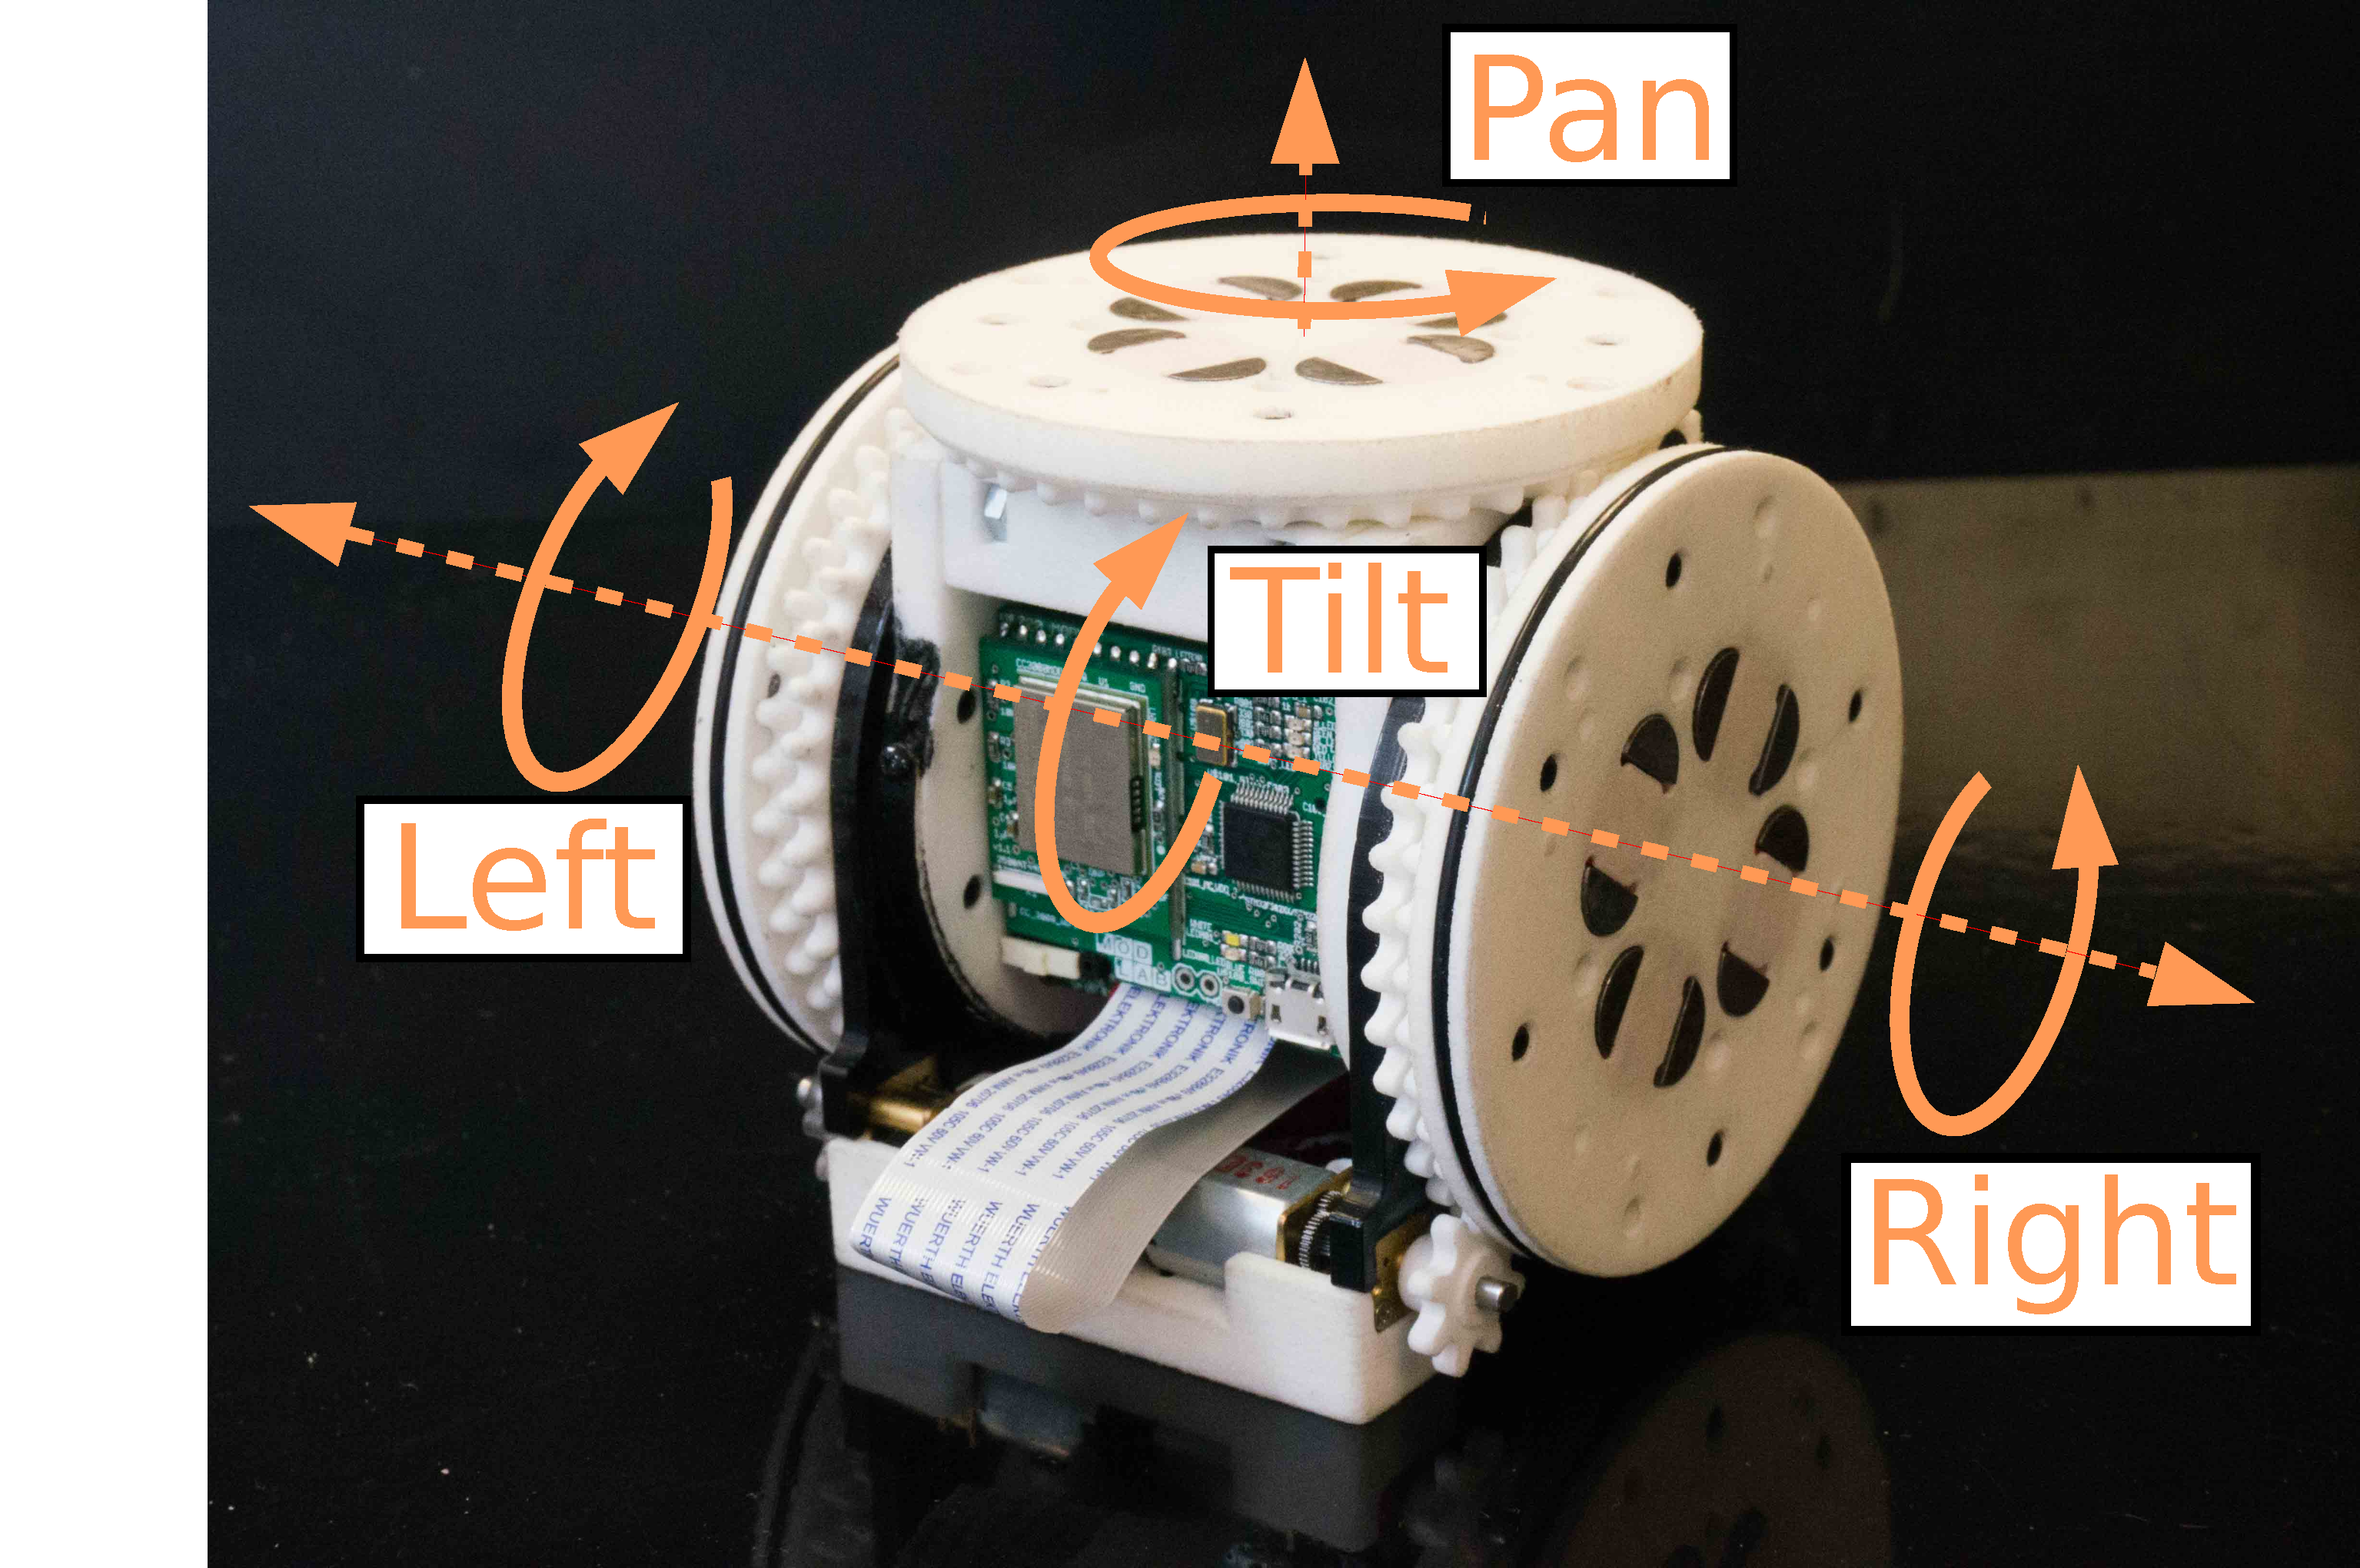
\includegraphics[height=1.5in]{images/smores_dof.pdf}
%\end{center}
%\caption{SMORES-EP module}
%\label{fig:smores-module}
%\vspace{-2em}
%\end{figure}
%

%\subsection{Brain Module} % (fold)
\label{sec:sensor_module}
%
Our system architecture assumes there is a single \textit{sensor module}, containing sensors and a computer, that is carried by a cluster of modules.
%SMORES-EP modules have no sensors that allow them to gather information about their environment. To enable autonomous operation, we extend the SMORES-EP hardware by introducing a \textit{sensor module}, shown in Figure~\ref{fig:sensor-module}.
The sensor module used in our experiments was designed to work well with SMORES-EP, and is shown in Figure~\ref{fig:sensor-module}.
The body of the sensor module is \TODO{get
dimensions}, and has thin steel plates on its front and back that allow SMORES-EP modules
to connect to it.
Computation is provided by an UP computing board with an Intel Atom 1.92 GHz
processor, 4 GB memory, and a 64 GB hard drive. A USB WiFi adapter provides
network connectivity. A front-facing Orbecc Astra Mini camera provides RGB-D
data, enabling the robot to explore and map its environment and recognize
objects of interest.  A thin stem extends $30cm$ above the body, supporting a
downward-facing webcam. This camera provides a view of a  $1m\times0.75m$ area
in front of the brain module, and is used to track AprilTag
\cite{olson2011apriltag} fiducials for reconfiguration. A $7.4v$, $2200mAh$ LiPo
battery provides about one hour of running time.

The decision to use a single centralized sensor module, rather than many sensors
distributed among all the modules, is an important aspect of our system
architecture, allowing us to use a single, powerful sensor that enabled SLAM,
navigation, and environment characterization. \TODO{expand on this, and maybe
move it to the sensing section.}

%
% Sensor Module Figure
\begin{figure}
\begin{center}
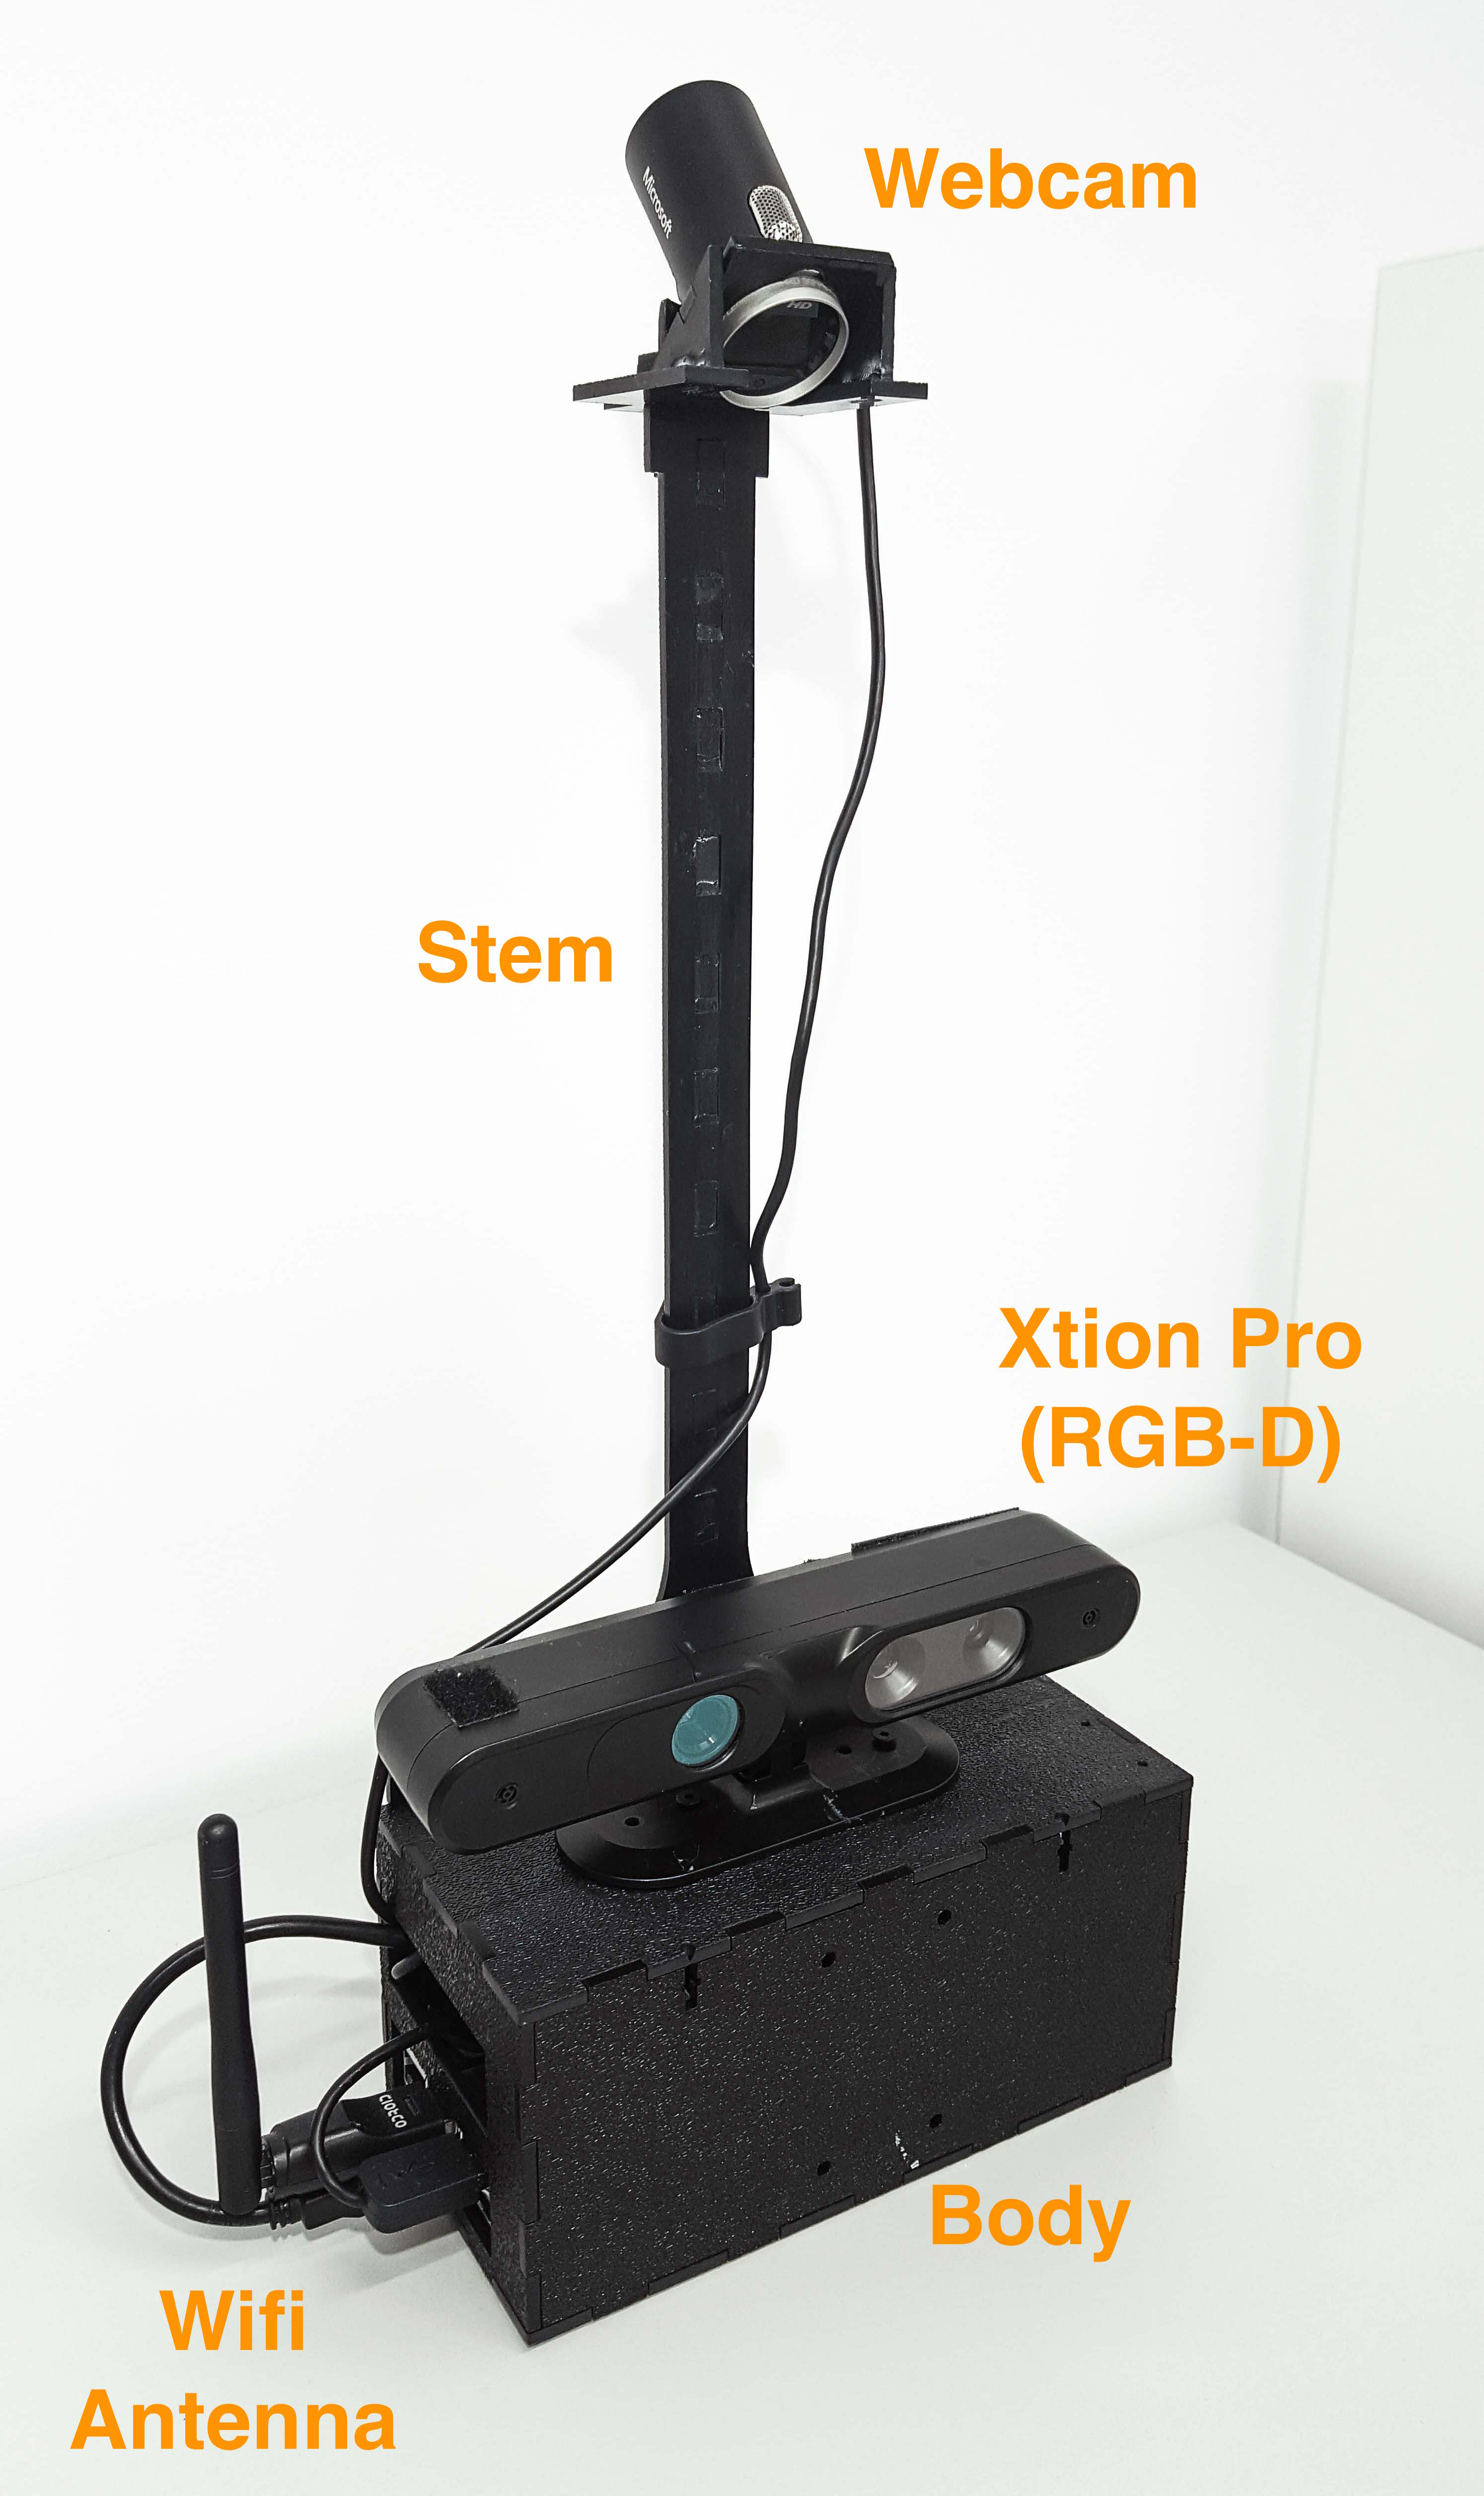
\includegraphics[width=0.3\textwidth]{images/sensor_module2.jpg}
\caption{Brain Module with labelled components.  UP board and battery are inside the body. \TODO{Change picture to new sensor.}}
\label{fig:sensor-module}
\end{center}
\vspace{-2em}
\end{figure}
%
%     __  ___       __          __                   __
%    / / / (_)___ _/ /_        / /   ___ _   _____  / /
%   / /_/ / / __ `/ __ \______/ /   / _ \ | / / _ \/ /
%  / __  / / /_/ / / / /_____/ /___/  __/ |/ /  __/ /
% /_/ /_/_/\__, /_/ /_/     /_____/\___/|___/\___/_/
%         /____/
%%
\subsection{High-Level Planner}
\label{sec:high-level}

In our architecture, the high-level planner subsystem provides a framework for users to specify tasks  at a high level using a formal language, and acts as the main, centralized controller that directs robot motion and actions based on the given tasks.
The high-level planner allows us to use each component of our system as a low-level atomic controller, and specify a wide-range of reactive robotic tasks as a set of high-level instructions using these controllers.

%\TODO{Jim, expand on / correct this. What aspects of the high level planner are general requirements of our architecture, and what aspects are specific to our implementation?}

%In this section, we will mainly discuss how we model our system in order to use LTLMoP to automatically generate a high-level controller for our desired robot task.

We abstract the robot and environment as a set of Boolean propositions.
For example, the robot action \textbf{pickUp} is \lt if the robot is currently picking up an object (and \lf otherwise) and the environment proposition \textbf{pinkItem} is \lt if the robot is currently sensing a pink item (and \lf otherwise).
LTLMoP supports a high-level language called Structured English that allows the robot task to be specified in terms of these propositions.
By using the library (Section~\ref{sec:configuration-specifics})  and environment characterization tools (Section~\ref{sec:environment-characterization}), these high-level statements are mapped to low-level sensing programs and robot controllers.
%To see how this works, consider Specification~\ref{spec:experiment}, which shows  high-level instructions from the user that direct the robot to explore a room, search, and move any object of interest to a drop-off zone.
The user specifies high-level robot actions in terms of behavior properties from the library. As discussed in Section~\ref{sec:configuration-specifics}, our system can choose to do a pick up action by executing any behavior from the library which has the behavior property \textbf{pickUp}, and which also satisfies the current environment characteristics. If the current robot configuration cannot execute an appropriate behavior, the robot will reconfigure to a different configuration that can.  In this way, the system autonomously chooses to implement  \textbf{pickUp}  appropriately in response to the sensed environment.
Propositions related to the state of the environment are evaluated using the perception tools described in Section~\ref{sec:exploration}. For example \textbf{pinkItem} is \lt if the robot is currently sensing a pink item, which is determined by consulting the color tracking functions.
%in Specification~\ref{spec:experiment}, the proposition \textbf{arrived} is \lt if the robot arrives at its target location, which is determined by consulting the robot's position in the map generated by SLAM. The proposition \textbf{dropoffZone} is \lt if the robot is currently sensing a drop-off zone, which is determined by consulting both the map and color tracking functions.

%The user specifies high-level robot actions in terms of behavior properties from the library.  For example, Line 7 in Specification~\ref{spec:experiment} specifies that under certain conditions, the robot should do \textbf{pickUp}.  As discussed in Section~\ref{sec:configuration-specifics}, our system can choose to do \textbf{pickUp} by executing any behavior from the library which has the behavior property \textbf{pickUp}, and which also satisfies the current environment characteristics. If the current robot configuration cannot execute an appropriate behavior, the robot will reconfigure to a different configuration that can.  In this way, the system autonomously chooses to implement  \textbf{pickUp}  appropriately in response to the sensed environment.

%Some robot actions, such as \textbf{driveExplore}, \textbf{driveToObject}, and \textbf{driveToDropoff}, requires the robot to navigate in the environment without colliding with obstacles.
%To achieve this, a goal pose is first determined by the controller and sent to a path planning program to generate a collision free path while considering the dynamics of the robot.
%The path is then converted to a sequence of robot velocity vectors and used as the input to control a parametric driving behavior in the library.
%In this work, we use the ROS navigation package\footnote{http://wiki.ros.org/navigation} to generate paths for a differential drive robot to control the ``Tank'' configuration in the library.

%Propositions related to the state of the environment are evaluated using the perception tools described in Section~\ref{sec:exploration}. For example in Specification~\ref{spec:experiment}, the proposition \textbf{arrived} is \lt if the robot arrives at its target location, which is determined by consulting the robot's position in the map generated by SLAM. The proposition \textbf{dropoffZone} is \lt if the robot is currently sensing a drop-off zone, which is determined by consulting both the map and color tracking functions.

%\begin{spec}[h!]
%\caption{Search and move any object of interest to the drop-off zone}
%\label{spec:experiment}
%\vspace{-0.1cm}
%\small\setlength{\jot}{0pt}
%\begin{fleqn}[3pt]
%\leqnomode
%\begin{subequations}
%\renewcommand{\theequation}{\arabic{equation}} 
%\makeatletter
%\renewcommand\tagform@[1]{\maketag@@@{\ignorespaces#1\unskip\@@italiccorr}}
%\makeatother
%\hskip-10cm
%\begin{alignat}{2}
%&\text{{\bf 1.} {\bf carry} is set on {\bf pickUp} and reset on {\bf drop}}&& \notag \\
%&\text{{\bf 2.} if you are not activating ({\bf pickUp} or {\bf drop} or {\bf driveToObject}}&& \notag \\
%&\hspace{1cm}\text{or {\bf driveToDropoff} or {\bf carry}) then do {\bf driveExplore}}&& \notag \\
%&\text{{\bf 3.} if you are activating {\bf carry} and you are not sensing }&& \notag \\
%&\hspace{1cm}\text{{\bf dropoffZone} then do {\bf driveExplore}}&& \notag \\
%&\text{{\bf 4.} do {\bf driveToDropoff} if and only if you are activating {\bf carry} }&& \notag \\
%&\hspace{1cm}\text{and you are sensing {\bf dropoffZone}}&& \notag \\
%&\text{{\bf 5.} do {\bf driveToObject} if and only if you are not activating {\bf carry} }&& \notag \\
%&\hspace{1cm}\text{and you are sensing {\bf object}}&& \notag \\
%&\text{{\bf 6.} do {\bf drop} if and only if you were activating {\bf driveToDropoff } }&& \notag \\
%&\hspace{1cm}\text{and you are sensing {\bf arrived}}&& \notag \\
%&\text{{\bf 7.} do {\bf pickUp } if and only if you were activating {\bf driveToObject} }&& \notag \\
%&\hspace{1cm}\text{and you are sensing {\bf arrived}}&& \notag \\
%&\text{{\bf 8.} infinitely often not {\bf carry}}&& \notag
%\end{alignat}
%\end{subequations}
%\end{fleqn}
%\vspace{-0.4cm}
%\end{spec}


Our implementation employs an existing framework called LTLMoP to automatically generate robot controllers from user-specified high-level instructions using formal methods \cite{DBLP:conf/iros/FinucaneJK10,DBLP:journals/trob/Kress-GazitFP09}.
Given a specification,  LTLMoP will synthesize a robot controller that satisfies the given  task (if one exists). The controller is synthesized in the form of a finite state automaton.
Each state specifies a set of high-level robot actions that need to be performed, and transitions between states are specified with a set of environment propositions.
Execution of the high-level controller begins at the predefined initial state in the finite state automaton. In each iteration, the values of all environment propositions are determined by calling the corresponding sensing program. Then, we determine the next state in the finite state machine by taking the transition that matches the current value of all environment propositions. 
In the next state, the specified high level behavior properties are mapped to a behavior from the design library which satisfies both the behavior properties and current environment type.

%Since the synthesized high-level controller is a discrete finite state automaton, we need to implement it continuously in order to control the robot to satisfy the given task.
%Execution of the high-level controller begins at the predefined initial state in the finite state automaton. In each iteration, the values of all environment propositions are determined by calling the corresponding sensing program. Then, we determine the next state in the finite state machine by taking the transition that matches the current value of all environment propositions. 
%In the next state, the specified high level behavior properties are mapped to a behavior from the design library which satisfies both the behavior properties and current environment type.
%The system then maps the system proposition specified in the next state to its set of behavior properties, and selects a behavior from the design library which satisfies both the behavior properties and current environment properties.
%If the robot is not currently in a configuration capable of executing the selected behavior, the system commands the robot to reconfigure. Finally, the behavior is executed, and the program continues on to the next iteration. 

%For example, in Fig.~\ref{fig:automaton} we start in the top state and execute the ``explore'' program.
%If  the robot senses a pink object, the value of ``pinkObject'' is \lt and therefore the next state is the bottom right state. We then stop the ``explore'' program and execute the ``driveToObject'' program.

%     ____                            __  _
%    / __ \___  _____________  ____  / /_(_)___  ____
%   / /_/ / _ \/ ___/ ___/ _ \/ __ \/ __/ / __ \/ __ \
%  / ____/  __/ /  / /__/  __/ /_/ / /_/ / /_/ / / / /
% /_/    \___/_/   \___/\___/ .___/\__/_/\____/_/ /_/
%                          /_/
\subsection{Perception and Planning for Information}
\label{sec:exploration}
%
%Our system provides a robust suite of perception algorithms to inform control and decision-making in unknown environments.  This suite of tools serves three major functions.  First, it enables exploration, allowing the robot to map its environment, localize, and avoid obstacles.  Second, it provides the capability to recognize objects and regions of interest related to the desired task.  Third, it provides functions that characterize environment properties, providing information that allows appropriate configurations and behaviors to be selected from the design library.

%Since the proposed system performs tasks in unknown environments and conditions, a robust suite of perception algorithms is required to inform control and decision-making. The robot must have the ability to explore and build a map of its environment while avoiding obstacles and tracking its pose. The system must be able to recognize objects and regions of interest related to the desired task. Finally, the system must characterize the environment in terms of configuration capabilities. Features in the environment may restrict which robot configurations can viably perform parts of the high-level task, such as retrieving an object or navigating to a waypoint. The system needs to recognize these features to be able to intelligently choose the appropriate robot configuration for performing the task.

The perception and exploration subsystem interprets sensor data to explore and understand its environment and inform robot behavior and adaptation. The architecture of this subsystem requires algorithms to perform SLAM, provide navigation goals for exploration, recognize objects of interest, and characterize the environment in terms of robot configuration abilities.

In our implementation, mapping and robot pose are provided by an RGB-D SLAM software package called RTAB-MAP\cite{rtabmap}. A 3D map of the environment is incrementally built and stored in an efficient octree-based volumetric map using Octomap\cite{octomap}. To drive exploration of the unknown environment, a Next Best View planner \cite{Daudelin2017} is used. Upon request, it provides waypoints to the high-level planner that maximize expected information collection of unknown regions of the environment. To identify objects of interest in the task, color detection and tracking is used.  Colored objects are recognized using CMVision\footnote{CMVision: http://www.cs.cmu.edu/$\sim$jbruce/cmvision/}, and tracked in 3D using depth information from the onboard 3D sensor\footnote{Lucas Coelho Figueiredo: https://github.com/lucascoelho91/ballFollower}. Although we implement object recognition by color, more sophisticated methods could be included in the same system architecture.

To enable the high-level planner to choose appropriate configurations for a task, our framework requires an environment characterization algorithm. This algorithm reasons about regions of interest in the environment to classify them in terms of the abilities of possible robot configurations. For our proof-of-concept, we implemented an algorithm that can differentiate between four environment types relevant to object manipulation, shown in Figure \ref{fig:characters}. 

When an object is recognized in the environment, the 3D information about its surroundings is evaluated. An occupancy grid is created around the object location, and all grid cells within a robot-radius of obstacles are denoted unreachable (as shown in Figure~\ref{fig:characterization}). The closest reachable point to the object within $20^o$ of the robot's line of sight to the object is selected. If the distance from this point to the object is greater than a threshold value and the object is on the ground, the environment is characterized as a ``tunnel'', likely requiring a configuration that is narrow enough to move between the surrounding obstacles to retrieve the object. If above the ground, the environment is characterized as a ``stairs'' environment, requiring a robot that can climb to reach the object. If the closest reachable point is under the threshold value, the environment is classified as either a ``free'' or ``sign'' environment, depending on the height of the colored object.

In addition to characterizing the environment, the algorithm also selects a waypoint based on the characterization for the robot to position itself for reconfiguration and performing the object manipulation task.

%
% Environment types figure
\begin{figure}[t]
      \centering
      \begin{subfigure}[t]{0.15\textwidth}
        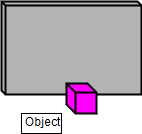
\includegraphics[width=\textwidth]{images/FreeEnvironment.png}
        %\label{fig:obja}
        \caption{\textbf{``free'}' environment}
    \end{subfigure} \ \ \ \ \ \
    \begin{subfigure}[t]{0.15\textwidth}
        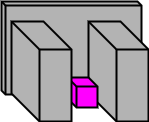
\includegraphics[width=\textwidth]{images/TunnelEnvironment.png}
        %\label{fig:objb}
        \caption{\textbf{``tunnel''} environment}
    \end{subfigure}
    
    \begin{subfigure}[t]{0.15\textwidth}
        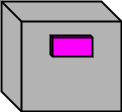
\includegraphics[width=\textwidth]{images/HighFreeEnvironment.png}
        %\label{fig:objb}
        \caption{\textbf{``sign''} environment}
    \end{subfigure} \ \ \ \ \ \
    \begin{subfigure}[t]{0.15\textwidth}
        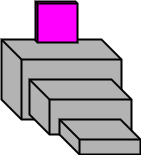
\includegraphics[width=\textwidth]{images/LedgeEnvironment.png}
        %\label{fig:objb}
        \caption{\textbf{``stairs''} environment}
    \end{subfigure}
      \caption{Environment characterization types.}
      \label{fig:characters}
   \end{figure}
%
% Characterization method figure
\begin{figure}
\begin{center}
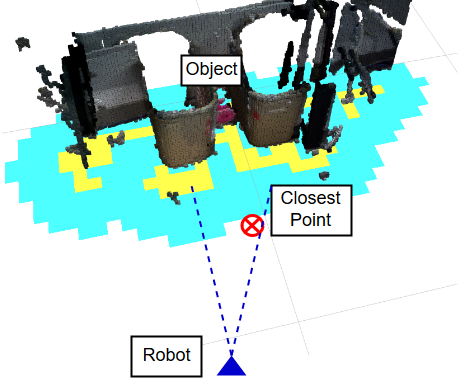
\includegraphics[width=0.4\textwidth]{images/characterization.png}
\caption{An example of a \textbf{tunnel} environment characterization. Yellow grid cells are occupied, light blue cells are unreachable resulting from bloating obstacles.}
\label{fig:characterization}
\end{center}
\vspace{-2em}
\end{figure}

%    ______            _____          _____                 _ _____
%   / ____/___  ____  / __(_)___ _   / ___/____  ___  _____(_) __(_)_________
%  / /   / __ \/ __ \/ /_/ / __ `/   \__ \/ __ \/ _ \/ ___/ / /_/ / ___/ ___/
% / /___/ /_/ / / / / __/ / /_/ /   ___/ / /_/ /  __/ /__/ / __/ / /__(__  )
% \____/\____/_/ /_/_/ /_/\__, /   /____/ .___/\___/\___/_/_/ /_/\___/____/
%                        /____/        /_/
\subsection{Library of Configurations and Behaviors}
\label{sec:configuration-specifics}
%
In our architecture, the full set of capabilities of the modular robot is encoded in a library of robot configurations and behaviors.  Each entry is labeled with  attributes that describe what it does, as well as the environment conditions under which it may be used. This allows the high-level planner  to match environment characterizations from\ the perception subsystem with the configuration and behavior that can perform the task in the current environment.

Our implementation relies on a framework first presented in \cite{Jing2016}, which we summarize here. In this framework, the entire modular robot system is treated as a single robot with capabilities defined by a library. A library entry is defined as $l = (C,B_C,P_e,P_b)$ where:
\begin{itemize}
\item $C$ is the robot \emph{configuration}, specified by the connected structure of the modules.
\item $B_C$ is a \emph{behavior} that $C$ can perform. A behavior is a controller that commands the robot to perform a specific useful action. 
\item $P_b$ is a set of \emph{behavior properties} that describes what $B_C$ does. 
\item $T_e$ is a set of \emph{environment types} that describe the environments in which this library entry is suitable. 
\end{itemize} 
%
When we specify tasks at the high level, we use behavior properties $P_b$ to describe a desired robot action without explicitly specifying a configuration or behavior.
Environment types $T_e$ specify the conditions under which a behavior can be used, and are determined through a sensing process described in the next section.
 
(\TODO{Do we need to add more entries? or should we remove the following paragraphs for space})
In this work, we create five library entries for two different configurations,
listed in Table~\ref{table:1}. This library was created to accomplish an object retrieval task (described in Section~\ref{sec:experiments}), but the library can be expanded to include more entries for other environments and tasks. Note that each library entry consists of a configuration with its available behaviors subject to restrictions in environment conditions. To characterize the environment in terms of these restrictions, we use a perception algorithm described in Section \ref{sec:environment-characterization}.

The ``Tank'' configuration shown in Figure~\ref{fig:dropoff} is capable of picking
up and dropping objects in a ``free'' environment (described in Section \ref{sec:environment-characterization}). In addition, the ``Tank'' configuration can locomote on flat terrain. It uses a parametric differential drive behavior to convert a desired velocity vector into motor commands (\textbf{drive} in Table \ref{table:1}).

The ``Proboscis'' configuration shown in Figure~\ref{fig:pink_grab} has
a long arm in front, and is suitable for reaching between obstacles in a narrow ``tunnel'' environment to grasp objects.
However, the locomotion ability of this configuration is limited to forward/backward
motion, making it unsuitable for general navigation.

This library-based framework allows us to specify tasks for modular robots at a high level, by associating abstract robot actions with robust low-level controllers that execute appropriate robot behaviors based on the sensed environment. For example, if a task specification requires the robot to execute a \textbf{pickUp} behavior, our system could select either the Tank or Proboscis configurations to perform the action, since both have behaviors property \textbf{pickUp}. To choose the appropriate configuration to use, the robot uses perception to characterize its environment in terms of the environment types $T_e$ associated with each configuration. If the environment is of type ``tunnel'', only the Proboscis configuration can be used, and the robot will take  reconfigure to form the Proboscis if it is not already in that configuration. Since self-reconfiguration is time-consuming, decisions are biased toward behaviors associated with the current configuration whenever possible, so that the robot only reconfigures when it is necessary to complete a task.
%
\begin{table}
\centering
\begin{tabular}{ |c|c|c| } 
 \hline
 \multirow{2}{6em}{Configuration} & Behavior & Environment \\
 & properties & Types \\
 \hline
 Tank & \textbf{pickUp} & ``free'' \\\hline
 Tank & \textbf{drop} & ``free'' \\\hline
 Tank & \textbf{drive} & ``free''\\ \hline
 Proboscis & \textbf{pickUp} & ``tunnel'' or ``free''\\ \hline
 Proboscis & \textbf{drop} &``tunnel'' or ``free'' \\ 
 \hline
\end{tabular}
\caption{A library of robot behaviors}
\label{table:1}
\vspace{-1em}
\end{table}

%     ____                        _____                        __  _
%    / __ \___  _________  ____  / __(_)___ ___  ___________ _/ /_(_)___  ____
%   / /_/ / _ \/ ___/ __ \/ __ \/ /_/ / __ `/ / / / ___/ __ `/ __/ / __ \/ __ \
%  / _, _/  __/ /__/ /_/ / / / / __/ / /_/ / /_/ / /  / /_/ / /_/ / /_/ / / / /
% /_/ |_|\___/\___/\____/_/ /_/_/ /_/\__, /\__,_/_/   \__,_/\__/_/\____/_/ /_/
%                                   /____/
\subsection{Reconfiguration}
\label{sec:reconfiguration}
%
When the high-level planner decides to use a new configuration during a task, the robot must reconfigure. Our system architecture allows any method for reconfiguration, provided that it requires no external sensing.  

SMORES-EP is capable of all three classes of modular self-reconfiguration (chain, lattice, and mobile reconfiguration) \cite{Davey2012,yim2003modular}.  We have implemented tools for mobile reconfiguration with SMORES-EP, taking advantage of the fact that individual modules can drive on flat surfaces as described in Section \ref{sec:hardware}.

Determining the relative positions of modules during mobile self-reconfiguration is an important challenge. 
%As discussed in Section~\ref{sec:related-work}, past systems have relied on offboard global positioning systems \cite{Paulos2015} or distributed approaches, in which sensors are mounted on each disconnected set of modules \cite{Yim2007}.  
Our localization method is centralized, using an RGB camera carried by the robot to track AprilTag fiducials mounted to individual modules.  As discussed in Section~\ref{sec:hardware}, the camera provides a view of a $1m\times0.75m$ \TODO{is this still correct?} area on the ground in front of the brain module.  
Within this area, our system provides pose for any module equipped with an AprilTag marker to perform reconfiguration. 
%Within this area (which we call the \emph{reconfiguration zone}), any module equipped with an AprilTag marker can detach from the cluster, drive to another location, and reattach to the cluster, provided that both of its wheels were in contact with the ground in its starting position.% \TODO{Get accurate number for height and FoV.}

%\subsection{Reconfiguration Procedure}
Given an initial configuration and a goal configuration, our reconfiguration controller commands a set of modules to disconnect, move and reconnect in order to form the new topology of the goal configuration. 
The robot first takes actions to establish the conditions needed for reconfiguration.  It begins by confirming that the reconfiguration zone is a flat surface free of obstacles (other than the modules themselves).  If the robot is carrying an object, it drops the object outside of the reconfiguration zone. It then  sets its joint angles so that all modules that need to detach have both of their wheels on the ground, ready to drive.
Then the robot performs operations to change the topology of the cluster by detaching a module from the cluster, driving, and re-attaching at its new location in the goal configuration, as shown in Figure~\ref{fig:reconf}.
Currently, reconfiguration plans are created by hand.  In the future, existing assembly planning algorithms (\cite{Werfel2007,Seo2013}) could be adapted to generate reconfiguration plans automatically.
Because the reconfiguration zone is free of obstacles, collision-free paths can be pre-computed and stored as part of the reconfiguration plan.
Once all module movement operations have completed and the goal topology is formed, the robot sets its joints to appropriate angles for the goal configuration to begin performing desired behaviors, and if necessary, the robot picks up any objects it dropped. This completes the reconfiguration process.

%The process consists of three stages: i) Pre-reconfiguration, ii) Module Movement, iii) Post-reconfiguration.

%\paragraph{Pre-reconfiguration} In the pre-reconfiguration stage, the robot takes actions to establish the conditions needed for reconfiguration.  It begins by confirming that the reconfiguration zone is a flat surface free of obstacles (other than the modules themselves).  If the robot is carrying an object, it drops the object outside of the reconfiguration zone. It then  sets its joint angles so that all modules that need to detach have both of their wheels on the ground, ready to drive. Once these conditions are established, module movement begins.

%\paragraph{Module Movement} During this stage, the topology of the cluster changes as a sequence of module movement operations are performed.  Each operation changes the topology of the cluster by detaching a module from the cluster, driving, and re-attaching at its new location in the goal configuration, as shown in Figure~\ref{fig:reconf}.

%In order to transform from an initial configuration to a goal configuration, a feasible reconfiguration plan (sequence of module movement operations) must be supplied before reconfiguration begins.  Each configuration in the library has an associated set of reconfiguration plans that allows it to transform to other configurations in the library.  Currently, reconfiguration plans are created by hand.  In the future, existing assembly planning algorithms (\cite{Werfel2007,Seo2013}) could be adapted to generate reconfiguration plans automatically.

% We denote a module movement operation as $MP=\left(m, m_d, m_a, f_m^d, f_m^a, f_{m_d}, f_{m_a}, \sigma \right)$ where:
% \begin{itemize}
% \item $m$ is the module whose location will be changed in this module operation.
% \item $m_d$ is the module that connects with $m$ before the operation.
% \item $m_a$ is the module that connects with $m$ after the operation. Notice $m_d$ and $m_a$ can be the same module. 
% \item The face $f_m^d$ of module $m$ connects with the face $f_{m_d}$ of module $m_d$ before the operation.
% \item The face $f_m^a$ of module $m$ connects with the face $f_{m_a}$ of module $m_a$ after the operation. Notice $f_m^d$ and $f_m^a$ can be the same face. In this work, we assume $f_m^a$ can only be the front or the back face of the module $m$.
% \item $\sigma$ is the path that module $m$ will follow during the operation.
% \end{itemize}

%To travel from its initial location to its final location, a module uses its left and right wheels to move by differential-drive.  Because the reconfiguration zone is free of obstacles, collision-free paths can be pre-computed and stored as part of the reconfiguration plan.  Paths can also be computed at runtime if desired.  AprilTag localization allows the robot to follow the path.

%Several techniques were developed to ensure reliable connection and disconnection during reconfiguration.  When a module disconnects from the cluster, the electro-permanent magnets on the connected faces are turned off.  To guarantee a clean break of the magnetic connection, the disconnecting module bends its tilt joint up and down, mechanically separating itself from the cluster. During docking, accurate alignment is crucial to the strength of the magnetic connection \cite{tosun2016design}.  For this reason, rather than driving directly to its final docking location, a module instead drives to a pre-docking waypoint directly in front of its docking location.  At the waypoint, the module spins in place slowly until its heading is perfectly aligned with the dock point, and then drives in straight to attach. To guarantee a good connection, the module intentionally overdrives its dock point, pushing itself into the cluster while firing its magnets.
%
\begin{figure}[t]
\begin{center}
  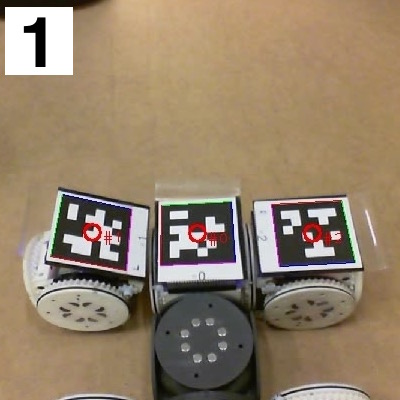
\includegraphics[width=0.32\columnwidth]{images/reconf_detach.jpg}
  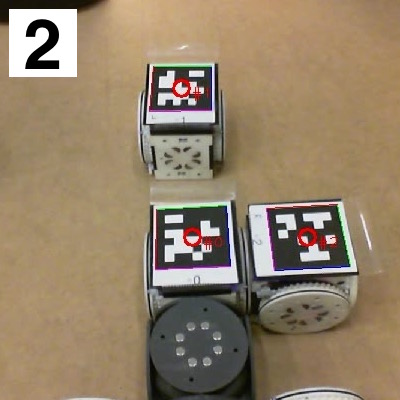
\includegraphics[width=0.32\columnwidth]{images/reconf_waypoint.jpg}
  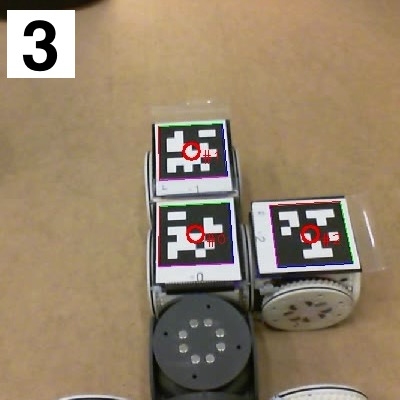
\includegraphics[width=0.32\columnwidth]{images/reconf_attach.jpg}
  \caption{Module movement during reconfiguration. (1) Left module detaches from cluster. (2) Module drives to waypoint, and spins to establish perfect heading. (2) Module drives straight in to dock point, and reattaches.}
  \label{fig:reconf}
\end{center}
\end{figure}

%\paragraph{Post-reconfiguration} Once all module movement operations have completed and the goal topology is formed, the robot sets its joints to appropriate angles for the goal configuration to begin performing desired behaviors, and if necessary, the robot picks up any objects it dropped. This completes the reconfiguration process. 


%     ______                     _                      __
%    / ____/  ______  ___  _____(_)___ ___  ___  ____  / /______
%   / __/ | |/_/ __ \/ _ \/ ___/ / __ `__ \/ _ \/ __ \/ __/ ___/
%  / /____>  </ /_/ /  __/ /  / / / / / / /  __/ / / / /_(__  )
% /_____/_/|_/ .___/\___/_/  /_/_/ /_/ /_/\___/_/ /_/\__/____/
%           /_/
\section{Experiment Results}
\label{sec:experiments}
%

As mentioned earlier, our work presents the first MSRR system that uses perception and reconfiguration to autonomously perform high-level tasks in unknown environments. We tested our system implementation on multiple, real-world tasks. These experiments accomplish two goals: First, they demonstrate our system's ability to autonomously adapt to multiple unknown environments and to complete different tasks. Second, they provide new observations of challenges with fully autonomous MSRR systems. These observations provide insight on what can be improved in autonomous MSRR systems to make them more robust and versatile.

Three experiments were run, each time varying the environment and the type of task to be performed. Each experiment required the robot to explore an unknown environment to search for and identify one or more objects of interest, and then complete some manipulation task with those objects.

\subsection{Experiment I}

The first experiment was designed to involve a long and complex task in order to fully demonstrate the robot's exploration, reconfiguration, and manipulation abilities. For this experiment, the robot is tasked with cleaning a messy graduate student office.  It is directed to explore the unknown office environment and search for any brightly-colored metal garbage that can be recycled.  Whenever it finds brightly colored metal objects, it should pick them up and bring them to a designated drop-off zone for recycling, which is marked with a blue square on the wall.

The high-level task consisted of three different types of sub-tasks: explore the environment, find and retrieve all metal objects, and deliver each to the drop-off zone. Figure \ref{fig:map} shows the environment layout used in the experiment, designed to represent a messy office. Two colored objects were placed in the environment: a green soda can was placed in the open (a ``free'' environment type), and a pink spool of wire was positioned in a narrow gap between two trash cans (a ``tunnel'' environment). Obstacles, environment types, and locations of the objects and drop-off zone were unknown to the robot \textit{a priori}.  Note that the object colors (pink and green) have no influence on environment characterization: in other words, the robot does not know that the pink object is in a ``tunnel''  before the experiment starts.

Five SMORES-EP modules, one Brain Module, and three passive cubes composed the robot for performing the task. The robot grasped objects using modules' electro-permanent magnets to attach to steel washers on the objects.
During the experiment, the high-level planner used the library of two configurations and five behaviors described in Section \ref{sec:configuration-specifics}.

% Map
\begin{figure}
\begin{center}
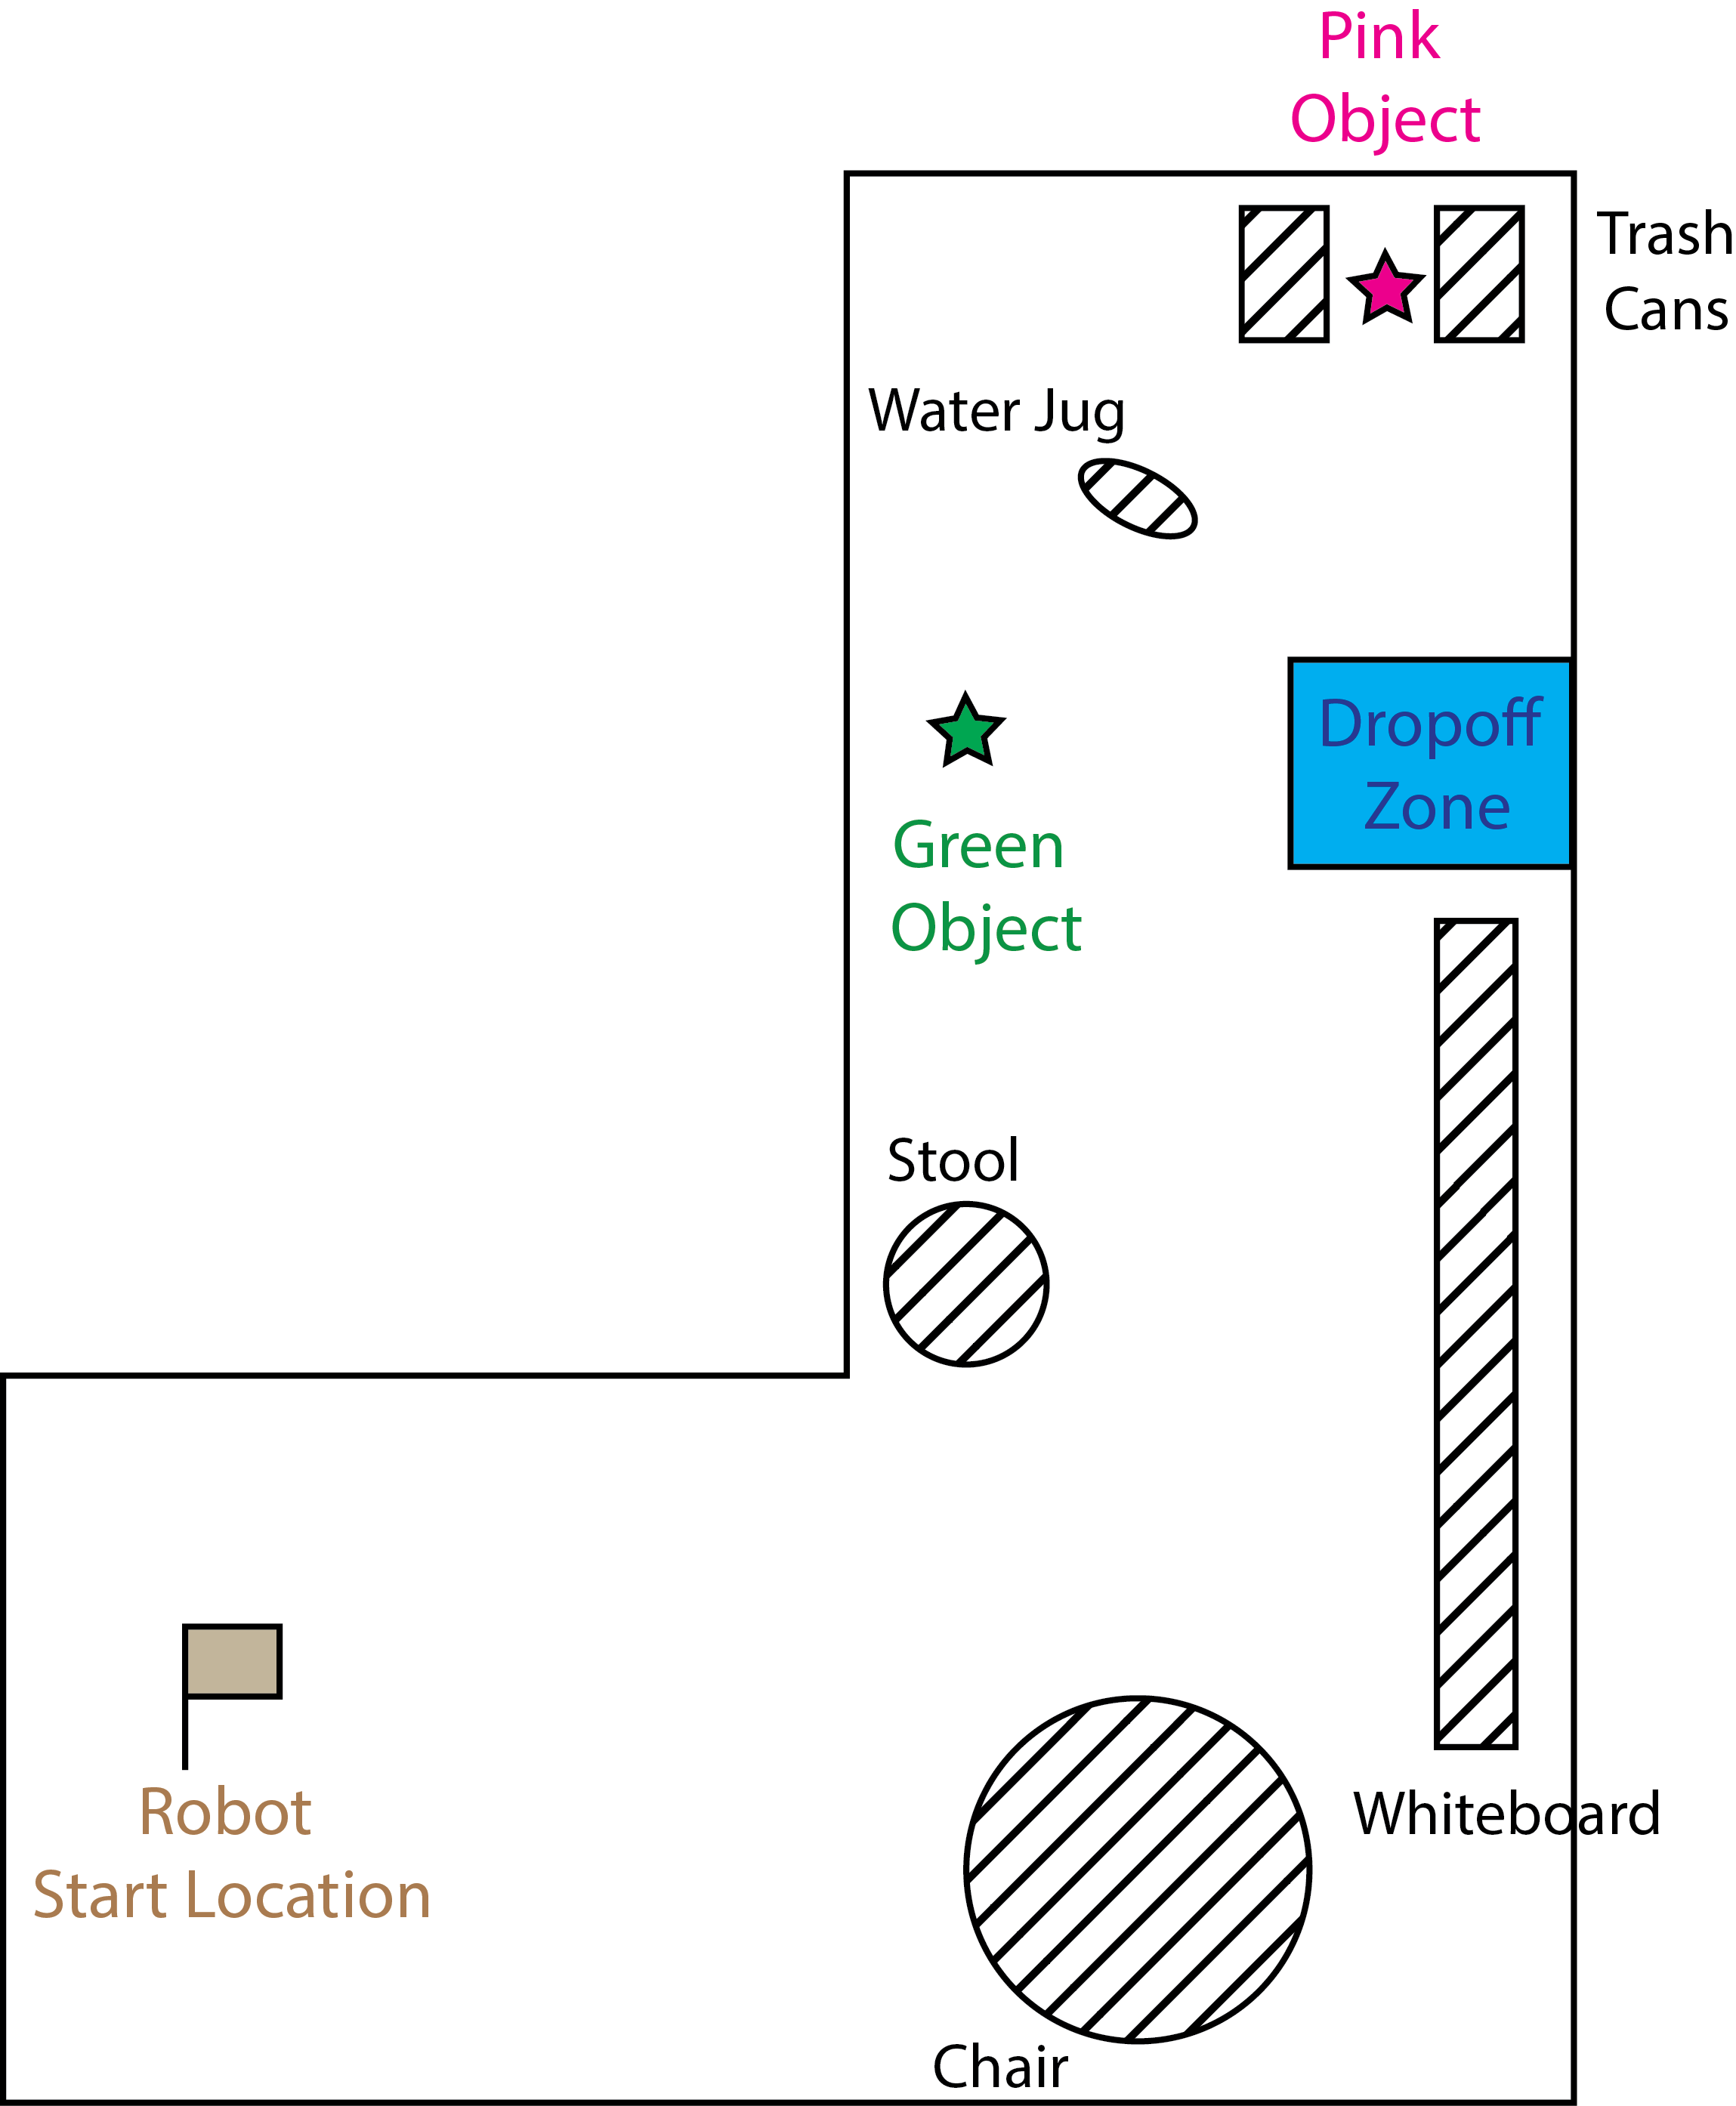
\includegraphics[width=0.3\textwidth]{images/RSSMap.png}
\caption{Diagram of Experiment I environment}
\vspace{-2em}
\label{fig:map}
\end{center}
\end{figure}

\begin{figure*}[t]
      \centering
      \begin{subfigure}[t]{0.32\textwidth}
        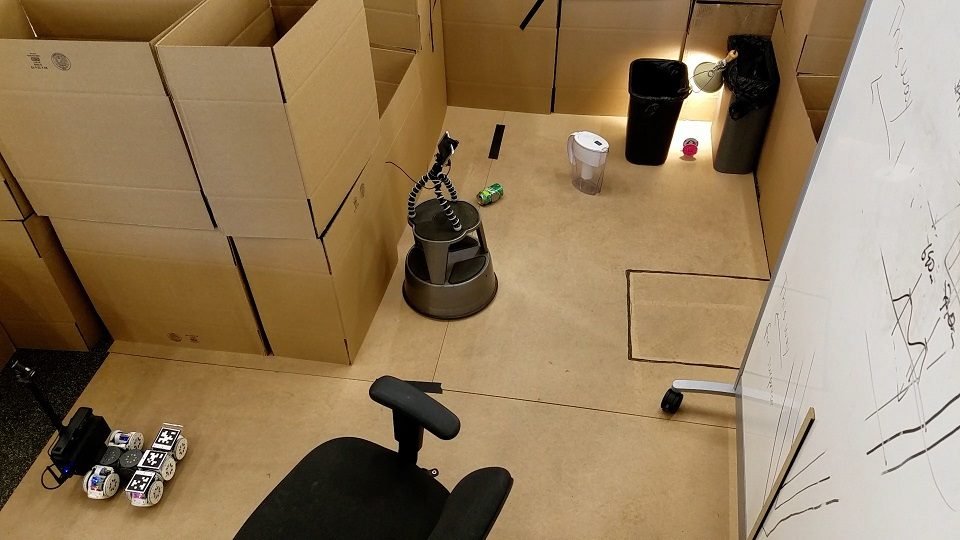
\includegraphics[width=\textwidth]{images/overhead_starting.jpg}
        %\label{fig:obja}
        \caption{Environment and robot starting location}
    \end{subfigure}
    \begin{subfigure}[t]{0.32\textwidth}
        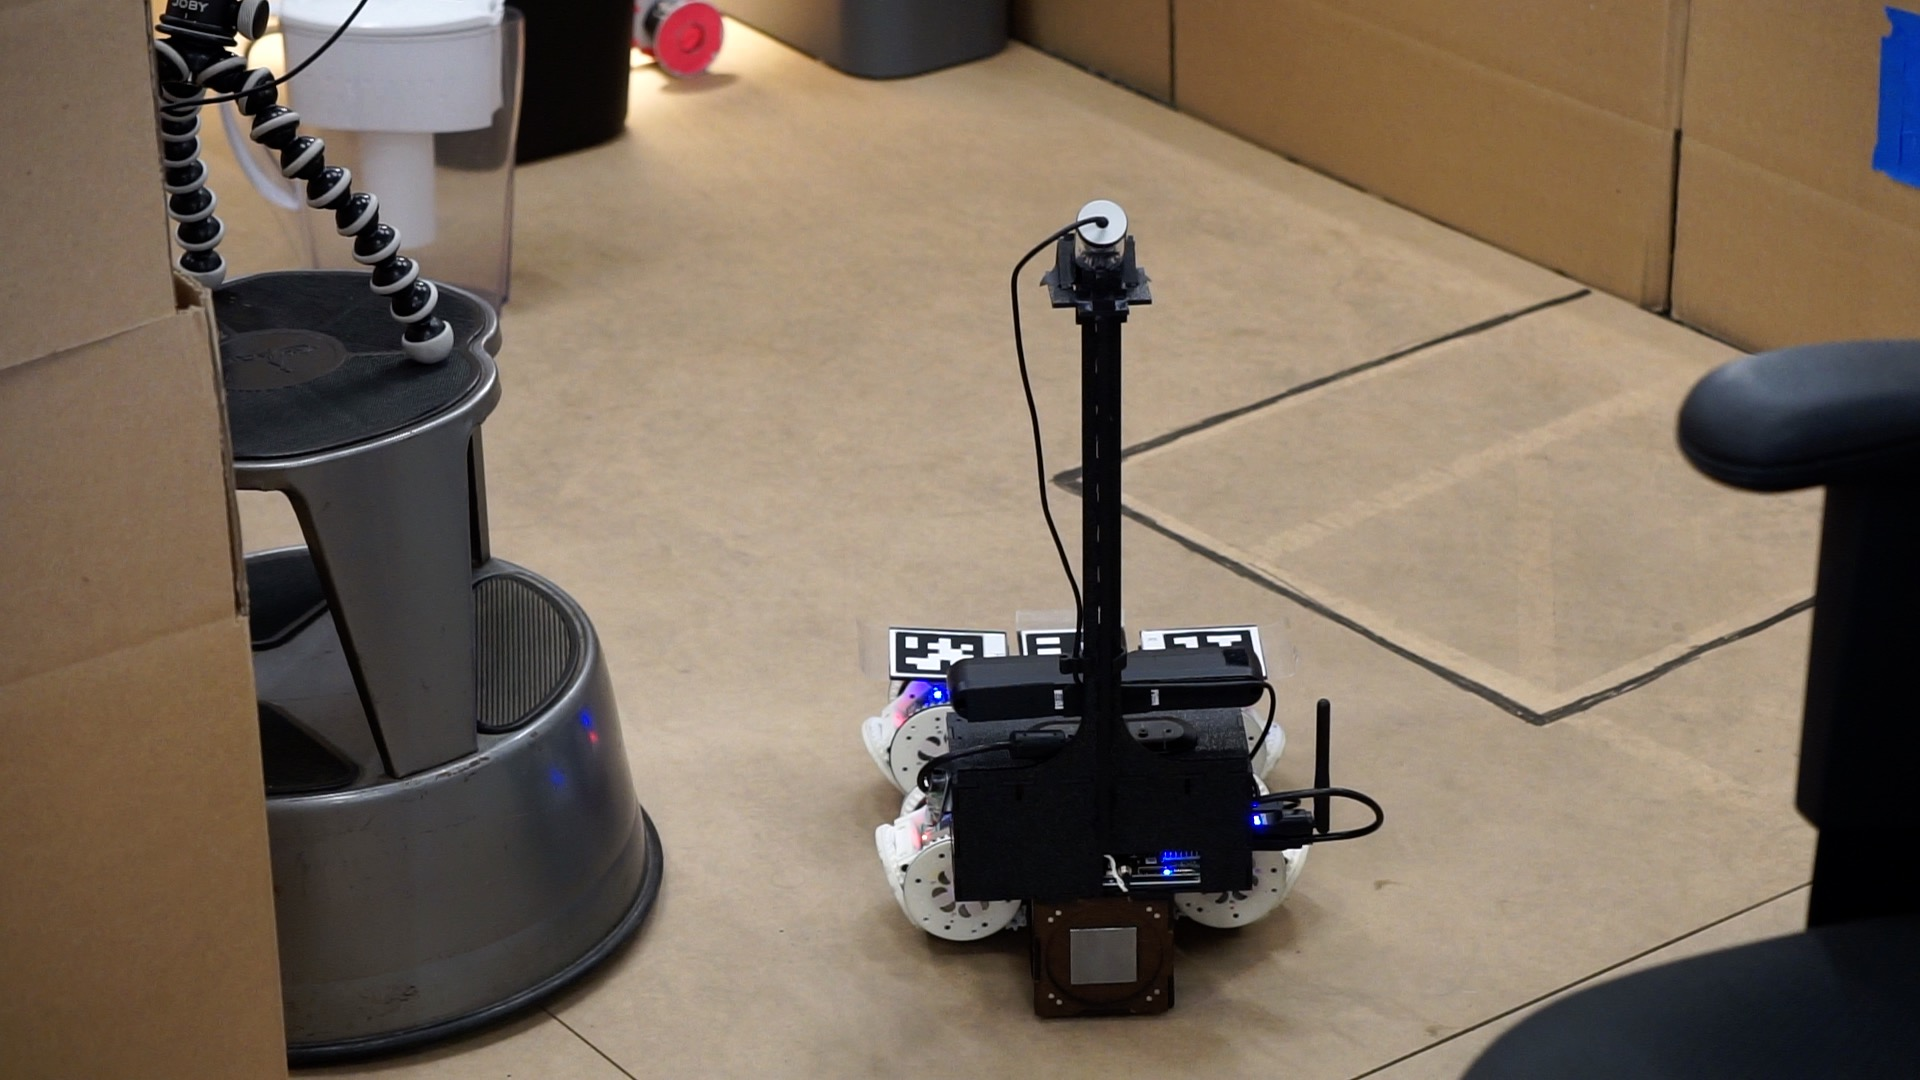
\includegraphics[width=\textwidth]{images/exploration.jpg}
        %\label{fig:objb}
        \caption{Exploring  while searching for objects}
    \end{subfigure}
    \begin{subfigure}[t]{0.32\textwidth}
        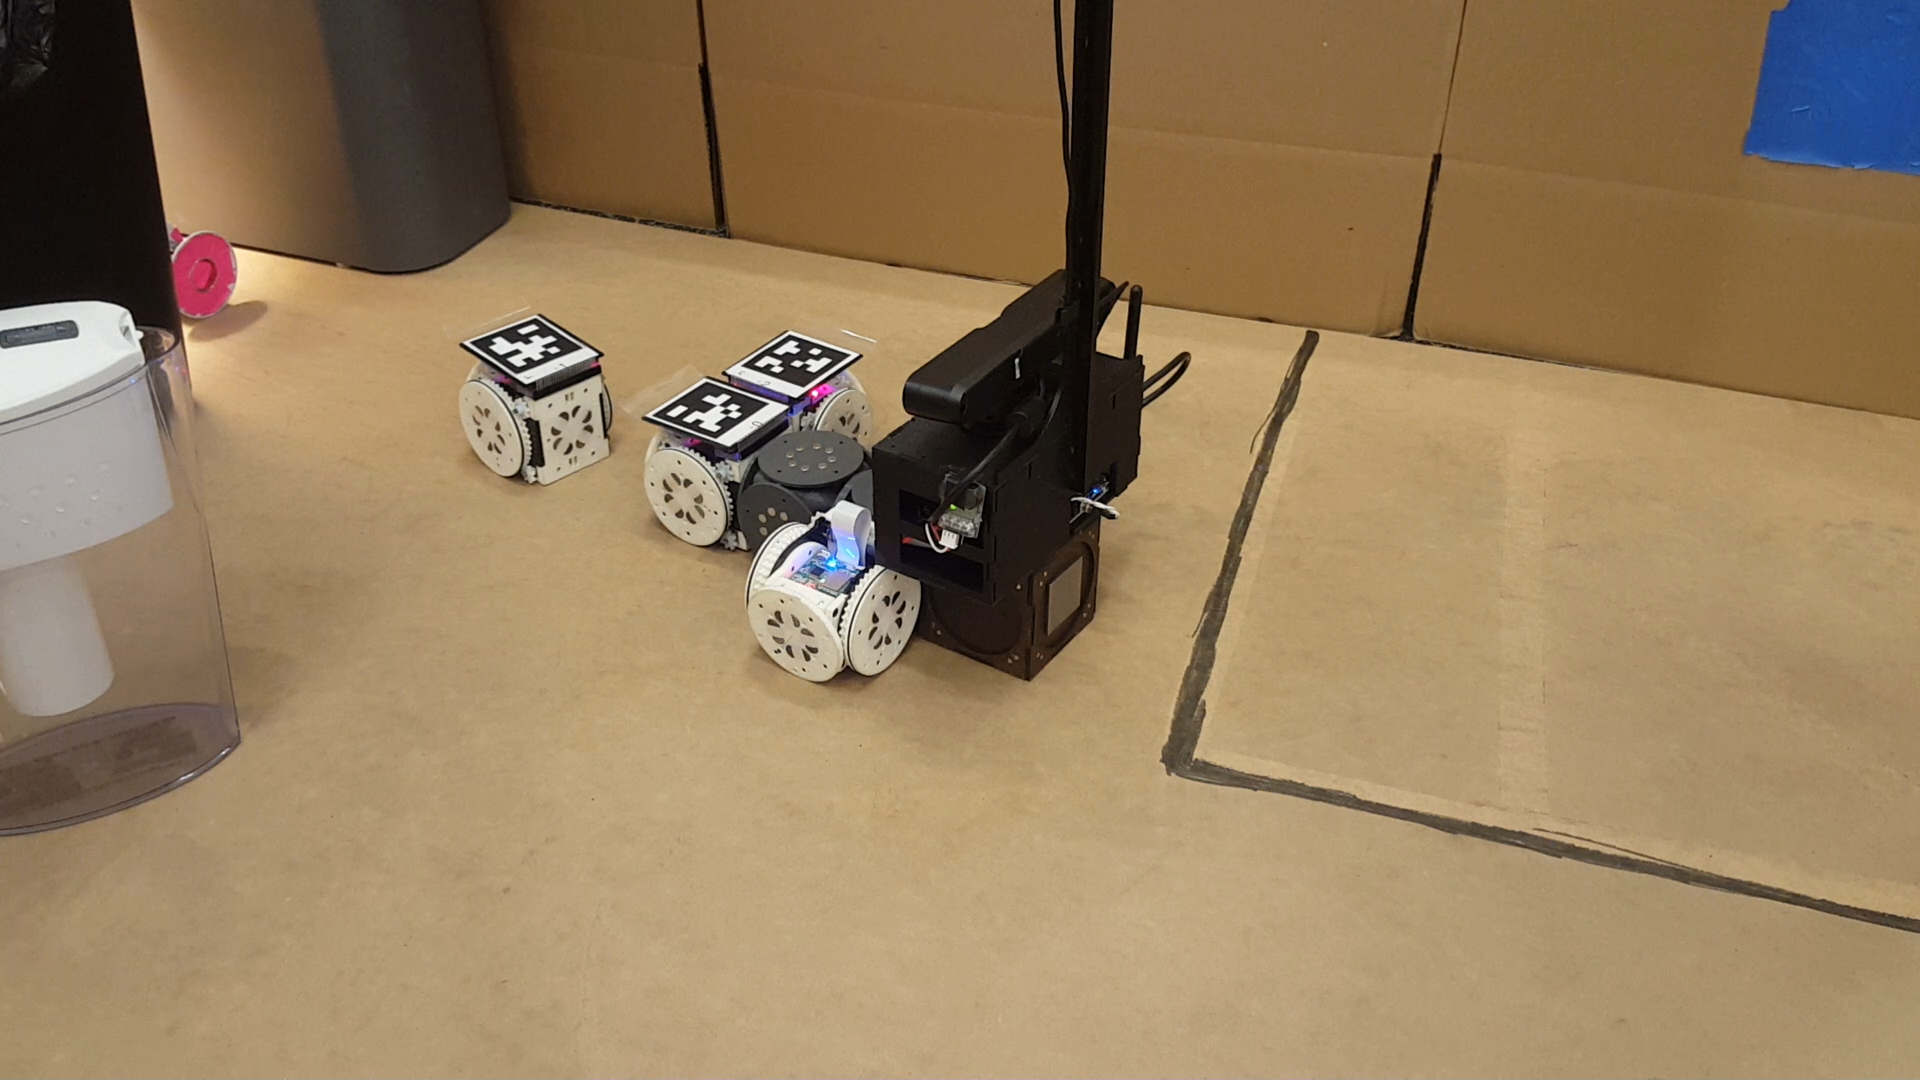
\includegraphics[width=\textwidth]{images/reconfiguration.png}
        %\label{fig:objb}
        \caption{Reconfiguring to retrieve pink object}
    \end{subfigure}
    \begin{subfigure}[t]{0.32\textwidth}
        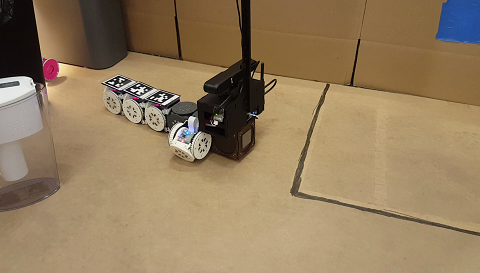
\includegraphics[width=\textwidth]{images/pink_retrieval.png}
        \caption{Retrieving pink object}
        \label{fig:pink_grab}
    \end{subfigure}
    \begin{subfigure}[t]{0.32\textwidth}
        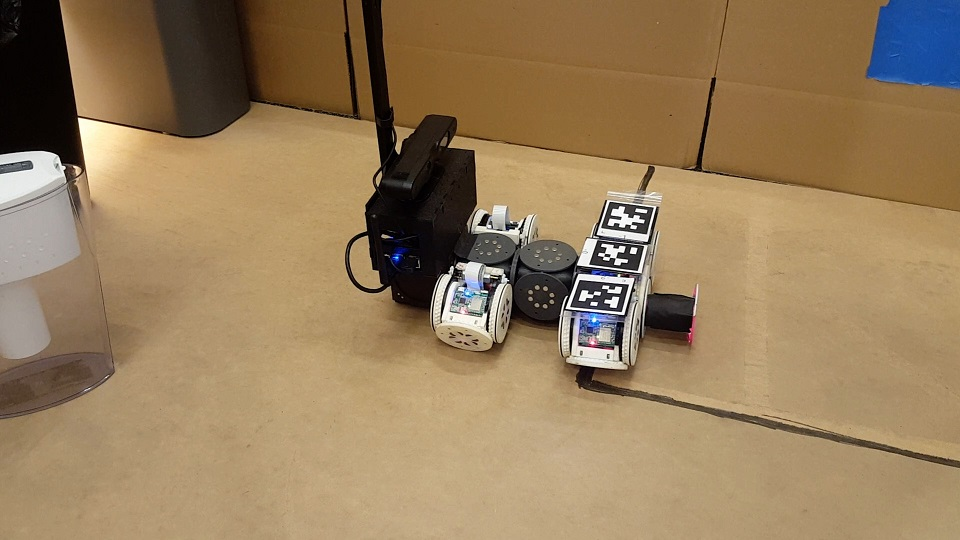
\includegraphics[width=\textwidth]{images/dropoff.jpg}
        \caption{Depositing an object in the drop-off zone}
        \label{fig:dropoff}
    \end{subfigure}
    \begin{subfigure}[t]{0.32\textwidth}
        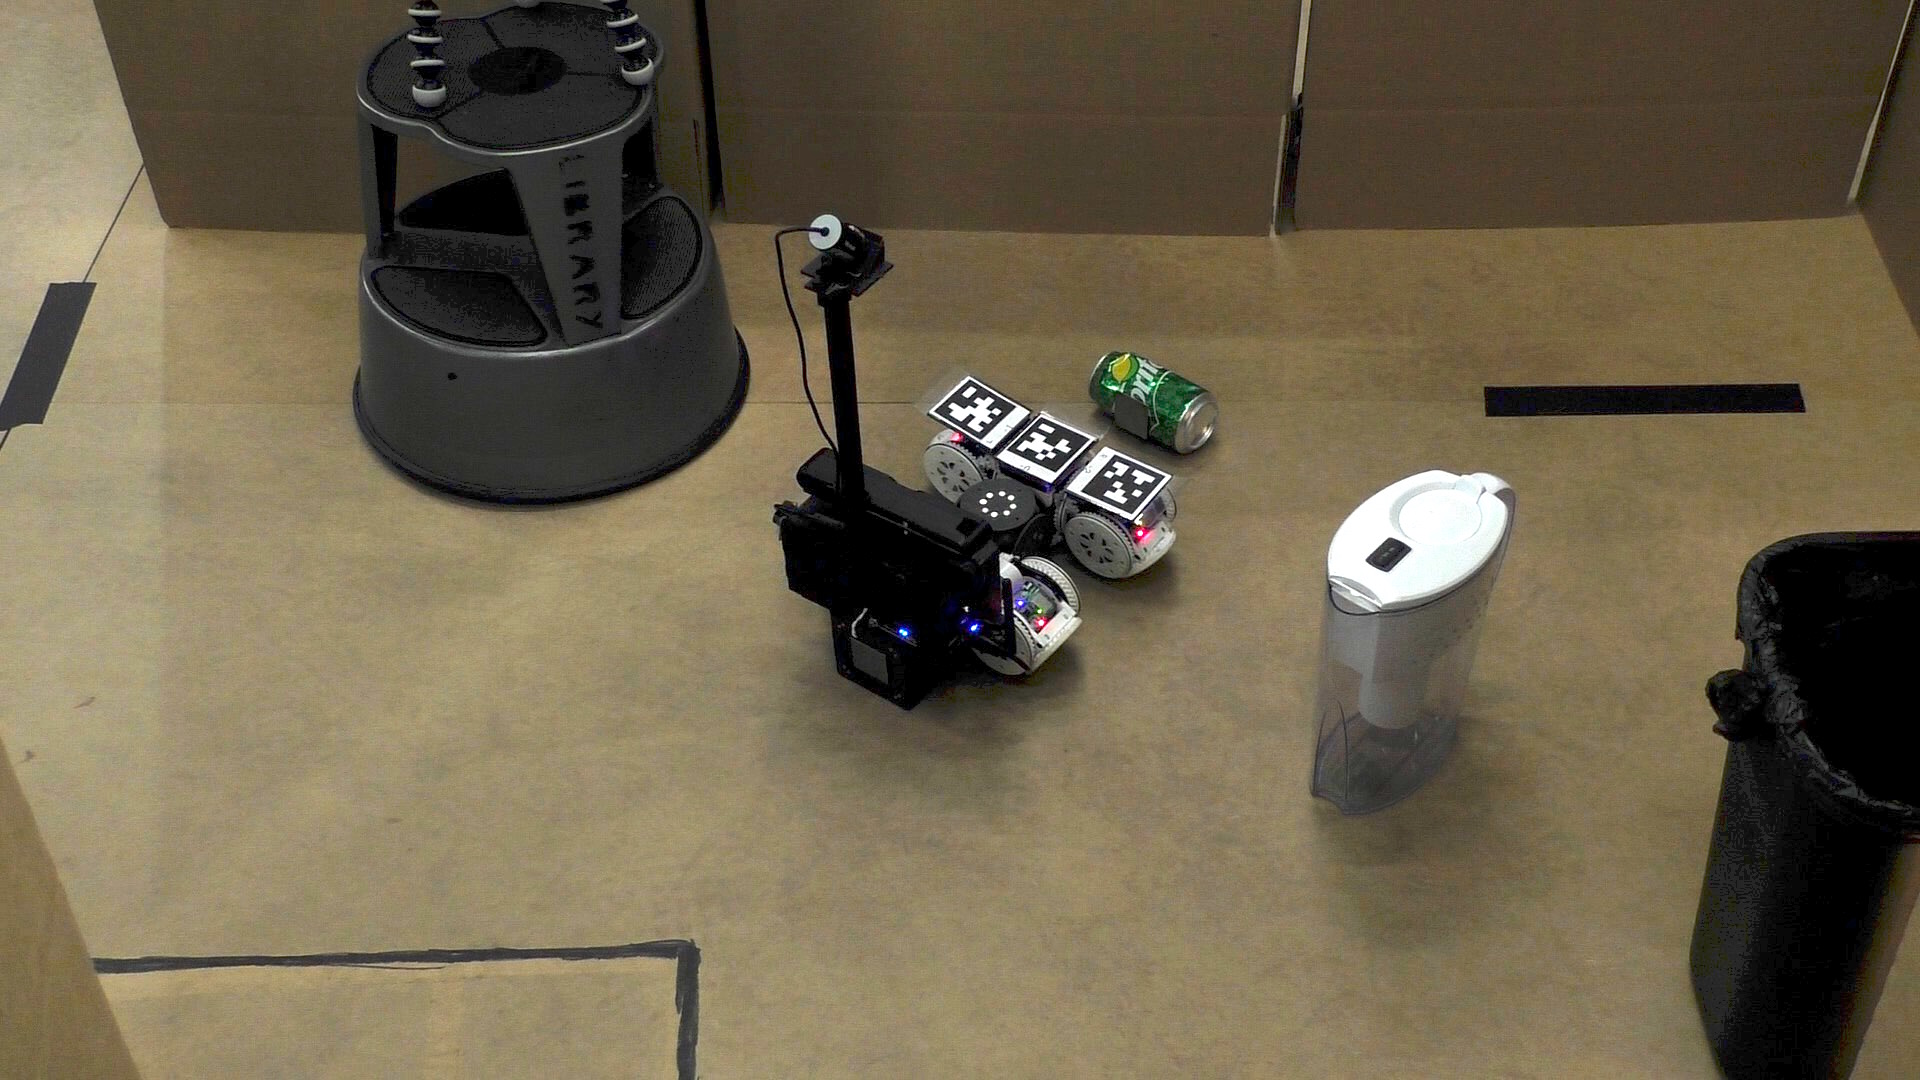
\includegraphics[width=\textwidth]{images/green_retrieval.jpg}
        %\label{fig:objb}
        \caption{Retrieving green object}
    \end{subfigure}
      \caption{Phases of Experiment I.}
      \label{fig:demo}
   \vspace{-1em}
   \end{figure*}
%
Figure \ref{fig:demo} shows snapshots from the experiment run. A video of the entire experiment is available as an attachment to this paper. The robot starts in the ``Tank'' configuration. The starting location prevented the robot from seeing the objects initially, forcing it to explore the environment to search for them. After a period of exploration, the robot locates the pink object. The characterization algorithm correctly classified the surrounding environment as a ``tunnel'' type, and accordingly the robot navigated in front of the object and reconfigured to the ``Proboscis'' configuration. The ``Proboscis'' then used its long arm to reach into the tunnel and pull the object out into the open.

 The ``Proboscis'' can only drive forwards and backwards (it cannot steer), so the robot concluded it needed to reconfigure back to the ``Tank'' to drive the object to the drop-off zone.  To do so, the robot dropped the object,  reconfigured, and picked the object back up. The ``Tank'' then navigated to and dropped off the object at the drop-off zone, which was previously located during exploration and recorded in the global map built by the SLAM algorithm.

 Once done, the robot navigated directly to the green object.  No further exploration was required since the green object was discovered while the robot was dropping off the pink object. The robot correctly determined
that the green object was in a ``free'' environment, and picked it up without reconfiguring. The robot finished the experiment by also delivering the green object to the drop-off zone. Figure \ref{fig:octomap} shows a volumetric map of the environment generated as the robot explored and delivered objects. The robot successfully completed all tasks in the experiment in about 26 minutes. 

Note that at one point in the video a human reaches onto the field to dislodge the green object from a crack in the floor.  This was due to a defect in the experimental setup (which is not supposed to have a crack in the floor) and not an error in the robot's performance.
%
\begin{figure}
\begin{center}
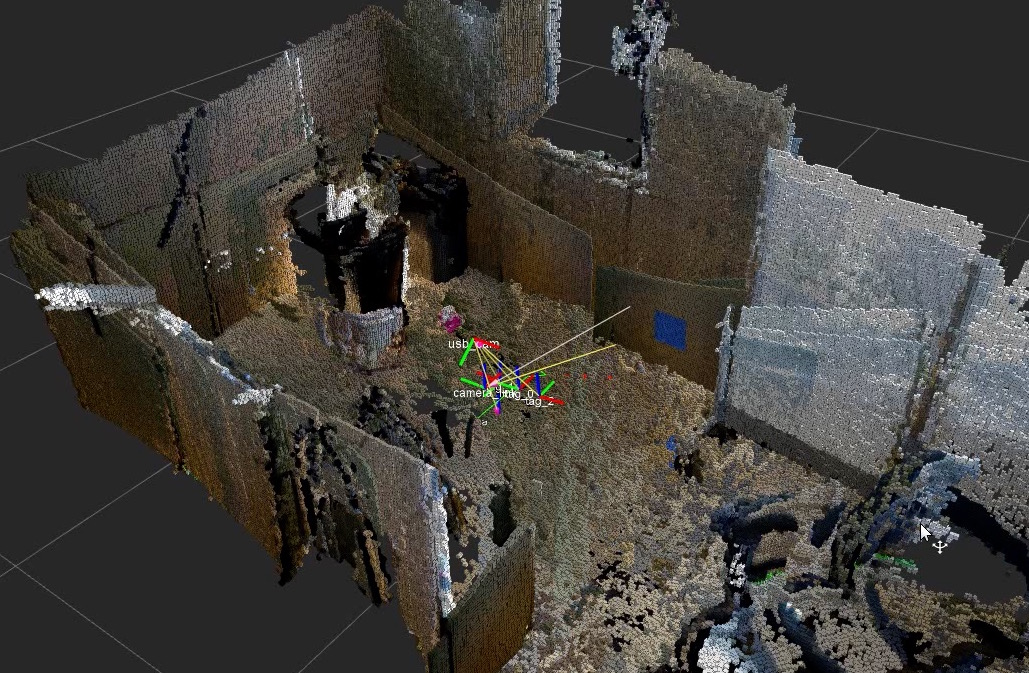
\includegraphics[width=0.4\textwidth]{images/map4.jpg}
\caption{Volumetric map of environment built by visual SLAM}
\vspace{-2em}
\label{fig:octomap}
\end{center}
\end{figure}

\subsection{Experiment II}

The second and third experiments were designed to demonstrate the breadth of our system's adaptive capabilities. As such, these two experiments included the same high-level task specification that is different from the task in Experiment I. However, differing environments between Experiment II and Experiment III force the robot to adapt differently to perform each experiment. For Experiment II, the robot is given a circuit that needs to be shipped, and is tasked with finding the shipping bin in which to place the circuit. A pink sign above the bin denotes the bin's location. The high-level task includes sub-tasks of exploring the unknown environment, locating and characterizing the environment surrounding the mail bin, and delivering the package to the bin.

Figure \ref{fig:exps}a shows the environment setup for Experiment II. The full performance of the experiment is included in the video attachment to this paper. Note that the mail bin has stairs in front of it, which the robot must climb in order to drop the circuit into the bin successfully. The robot begins the experiment in the ``scorpion'' configuration. Shortly after beginning exploration of the environment, the robot observes and recognizes the mailbox, and characterizes the environment surrounding it as ``high-free''. Based on this characterization, it determines that the ``snake'' configuration is needed to traverse the stairs. Using the 3D map and characterization of the environment surrounding the mail bin, the robot navigates to a point directly in front of the stairs, faces the bin, and reconfigures to the ``snake'' configuration. It then executes the stair climbing gait to reach the mail bin, and drops the circuit successfully. It then descends the stairs and reconfigures back to the ``scorpion'' configuration to end the mission.

\begin{figure}[t]
      \centering
      \begin{subfigure}[t]{0.24\textwidth}
        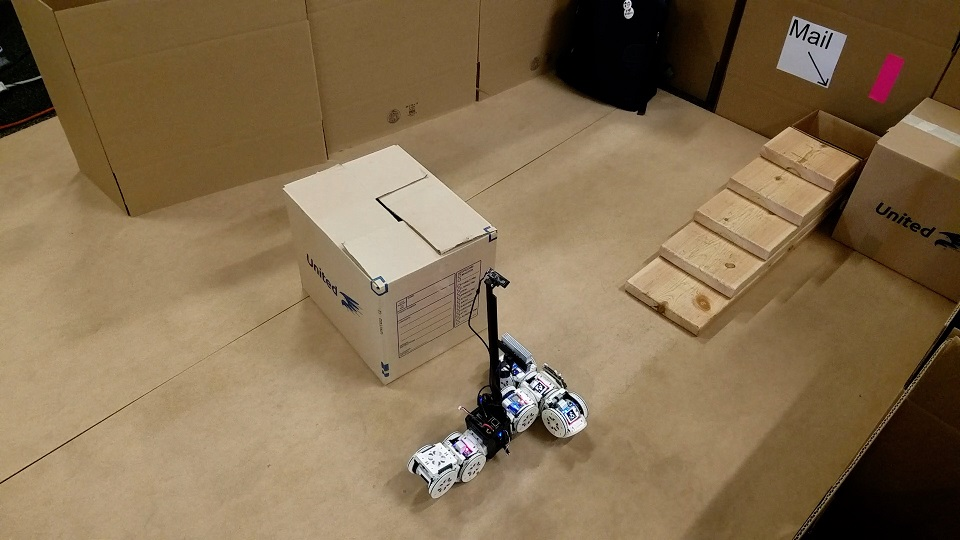
\includegraphics[width=\textwidth]{images/stairs_explore_overhead.jpg}
        %\label{fig:obja}
        \caption{Experiment II}
    \end{subfigure}
    \begin{subfigure}[t]{0.24\textwidth}
        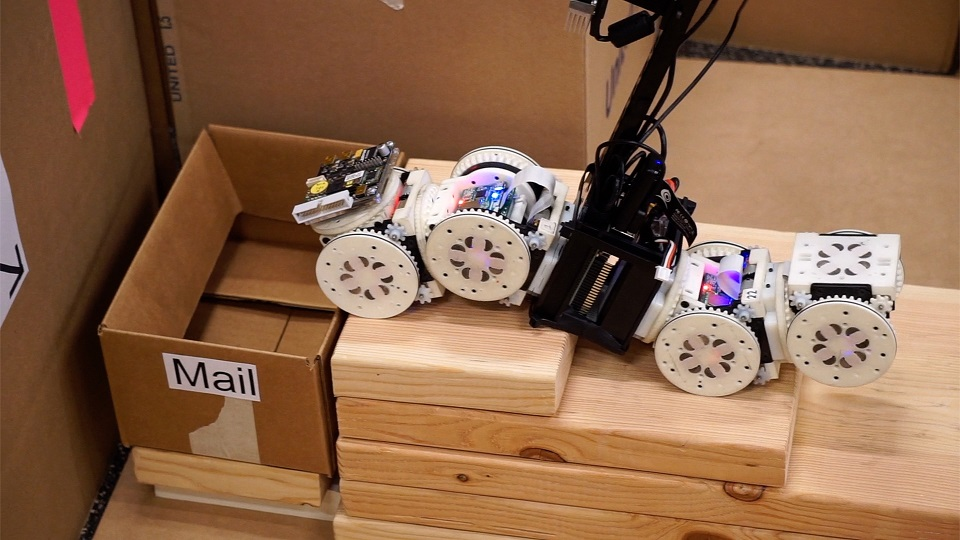
\includegraphics[width=\textwidth]{images/stairs_climb.jpg}
        %\label{fig:objb}
        \caption{Successful circuit delivery}
    \end{subfigure}
    
    \begin{subfigure}[t]{0.24\textwidth}
        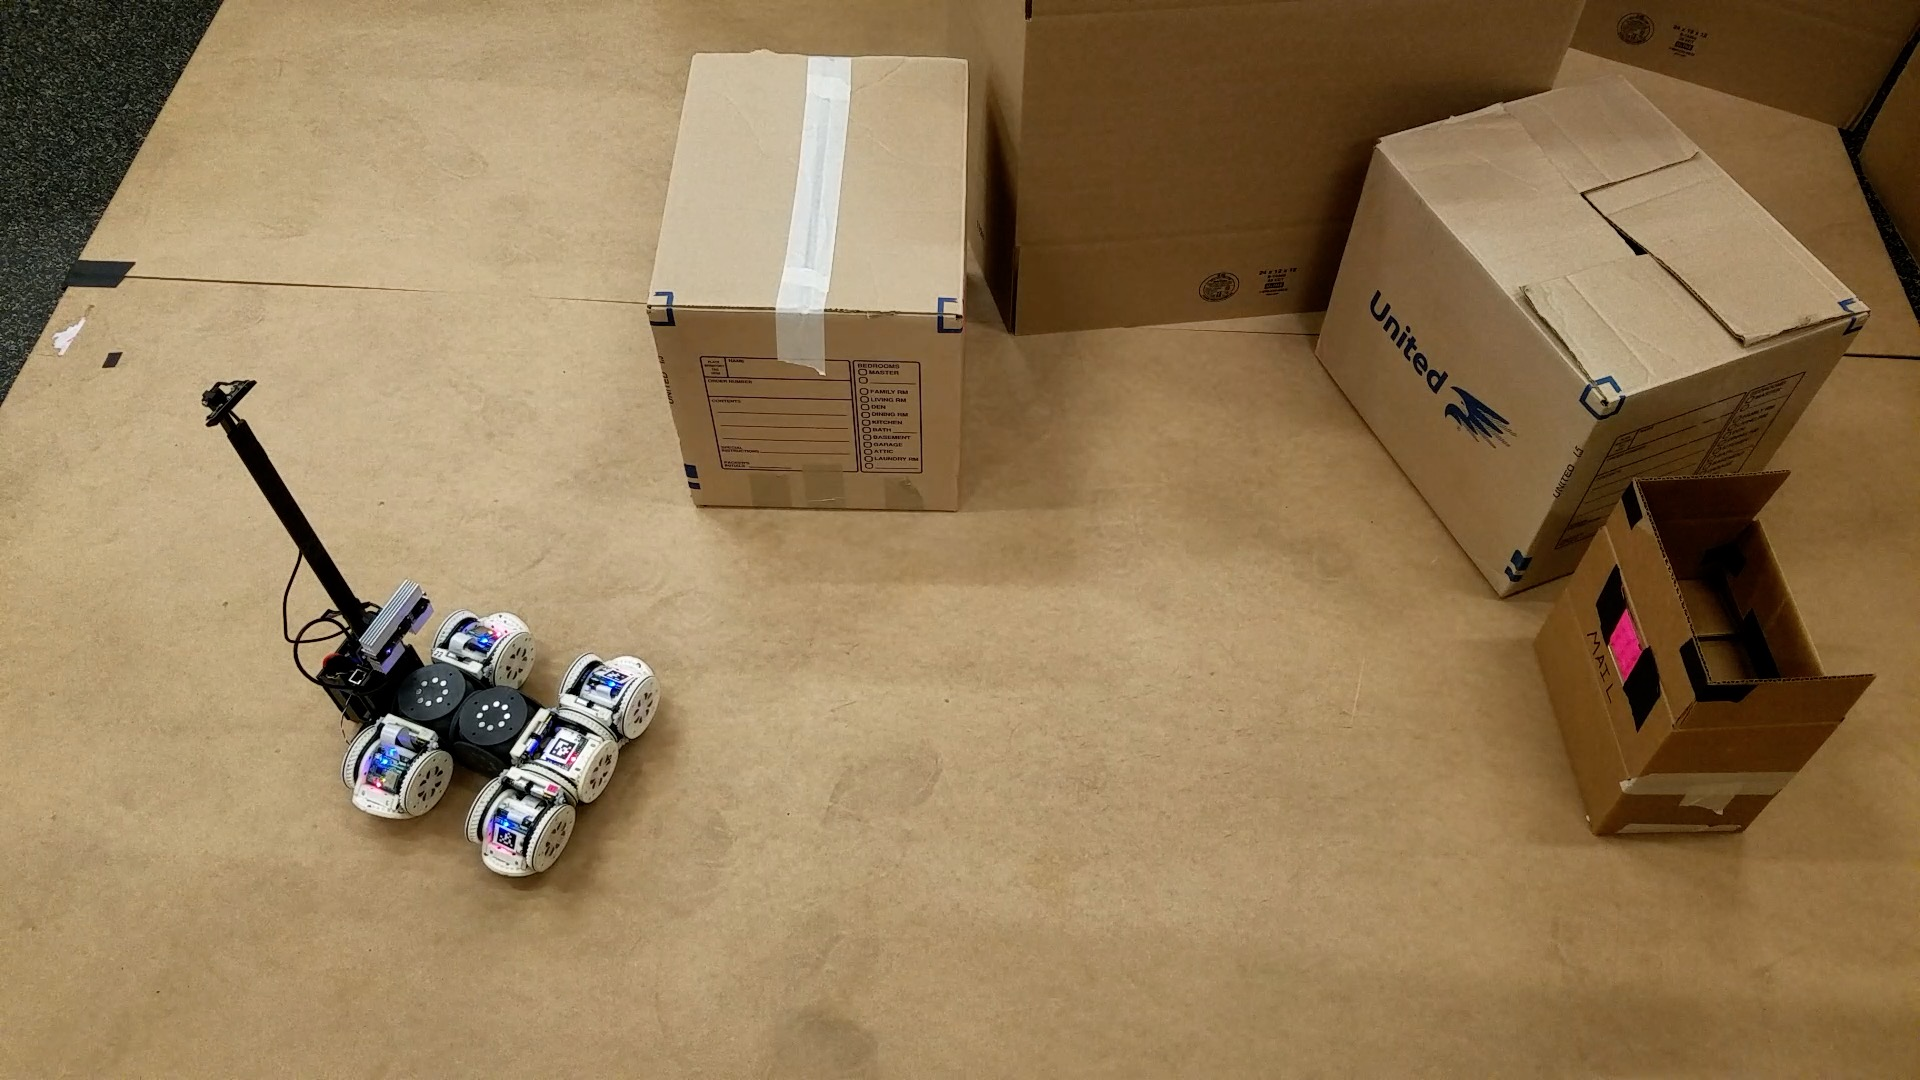
\includegraphics[width=\textwidth]{images/stamp_explore_overhead.jpg}
        %\label{fig:objb}
        \caption{Experiment III}
    \end{subfigure}
    \begin{subfigure}[t]{0.24\textwidth}
        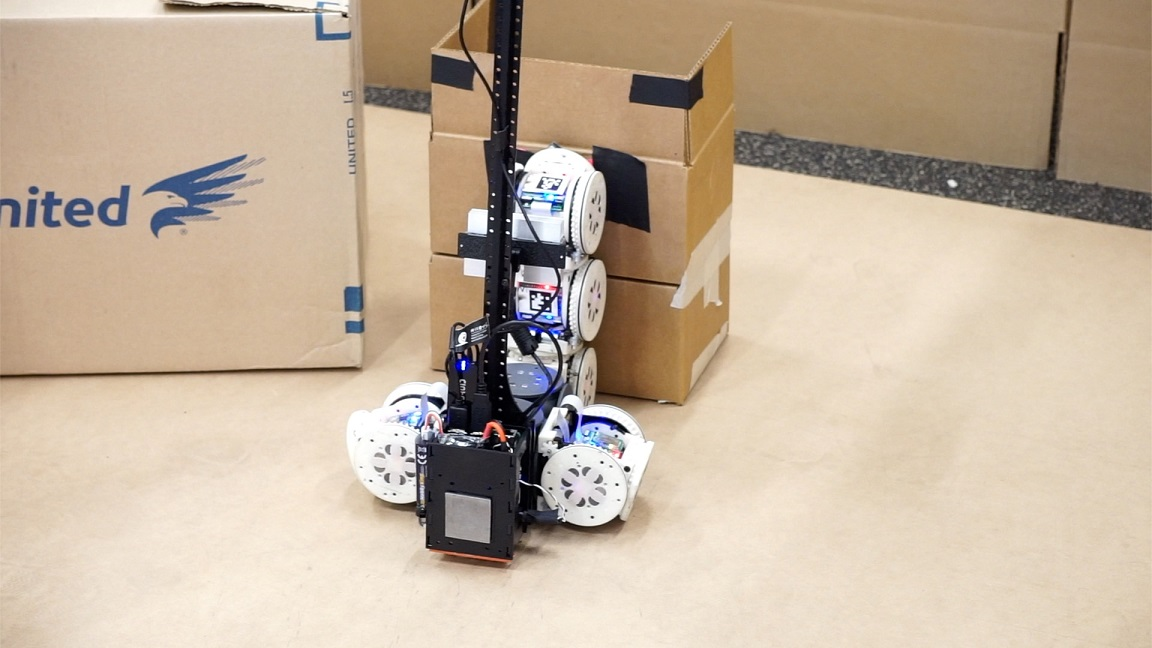
\includegraphics[width=\textwidth]{images/stamp_placing.jpg}
        %\label{fig:objb}
        \caption{Successful stamp placement}
    \end{subfigure}
      \caption{Experiments II and III.}
      \label{fig:exps}
   \end{figure}

\subsection{Experiment III}

For the final experiment, the robot is given a stamp and is tasked with placing it on a package that needs to be shipped. The high-level task has the same specification as in Experiment II, which for its environment includes the following sub-tasks: explore the unknown environment, find the package with stamp location denoted by a pink area, and place the stamp on the package. The robot was started in the ``tank'' configuration used in the first experiment.

Figure \ref{fig:exps}c shows the environment setup for Experiment III. Please see the video attachment for the full performance of this experiment. The robot begins exploring the unknown environment, and quickly observes the package to be stamped. It characterizes the environment as the ``stairs" environment using the 3D map created of the environment, and determines that the ``proboscis'' configuration is needed with the ``reaching'' gait to place the stamp on the pink goal area. The robot then navigates to a position directly in front of the package, reconfigures appropriately, and executes the gait to place the stamp correctly on the package to complete the task.

%     ____  _                           _
%    / __ \(_)___________  ____________(_)___  ____
%   / / / / / ___/ ___/ / / / ___/ ___/ / __ \/ __ \
%  / /_/ / (__  ) /__/ /_/ (__  |__  ) / /_/ / / / /
% /_____/_/____/\___/\__,_/____/____/_/\____/_/ /_/
\section{Discussion}
\label{sec:discussion}
We evaluate our system with respect to four criteria: \textit{autonomy}, \textit{capability}, \textit{reconfigurability}, and \textit{robustness}.
In all four areas, we evaluate both the  system \textit{architecture}, which is more general, and the system \textit{implementation}, which was actually used in our experiments.
%
\subsection{Autonomy}
%
\textit{How independent is the robot?  To what degree can it operate without external external computation, sensing, power, or other help?}

Autonomy was a major goal of this project, and an area in which the system architecture and implementation are both successful. Like most modular robots, the small size and strength of SMORES-EP made carrying
sensors and  computers  a challenge. Feasibility of implementation influenced our choice of system architecture: in contrast to the distributed sensing approaches used in prior modular work, our
decision to use a  centralized sensing architecture  allowed the robot to carry a  single, powerful sensor (the RGB-D
camera) enabling sophisticated capabilities like Visual SLAM and environment characterization. As a result, our implementation has more sensor-based autonomy than any previous modular robot.

Our implementation relies in part on external computation and wireless network access, but this is not a fundamental system requirement.   In fact,  in our implementation the majority of  heavy computation (mapping, navigation, video
processing) was done onboard on the sensor module, with a few processes (high-level planner, reconfiguration planner, and next-best-view planner) run offboard, primarily for development convenience. % 
In the future we believe everything could be run onboard with only minor adjustments.
%
\subsection{Capability}
%
\textit{  How capable is the implementation, in terms of solving real tasks? How general is the system architecture (does it place any limitations on
the kinds of tasks this system can address)? }

Broadly speaking, our system architecture provides the capability to \textit{specify high-level tasks}, \textit{gather information} about an unknown environment, \textit{move around the environment}, and \textit{interacting with the environment and objects within it}.  In theory, the architecture is capable of addressing any problem requiring these capabilities.

%{\color{red}(Specifying high-level tasks:)}
The high-level planner, environment characterization tools, and library work together to allow tasks to be represented in a flexible and reactive manner. For example, at the high level, experiments two and three are the same \textit{task:} deliver an object at a point of interest.  However, after characterizing the environment, the system determines that vastly different behaviors are required to complete the task, and in both cases, that reconfiguration is needed before the appropriate behavior can be performed. Similarly, in experiment 1 there is no high-level distinction between the green and pink objects - the robot is simply asked to \textit{retrieve} all objects it finds.  The sensed environment once again dictates the choice of behavior: the simple problem is solved in a simple way (green object), and the more difficult problem is solved in a more sophisticate way (pink object).

%{(\color{red} Gathering information:)}
The system's \textit{information-gathering} capability is largely dependent on the available sensing and computing hardware, and the algorithms used to process sensor data. We opted to use simple techniques for navigation, object recognition, and differentiating between environments, which were suitable for our proof-of-concept experiments.

To deploy a similar system in real life, more sophisticated techniques would need to be used.  Considering the ongoing trend towards high-performance sensors and computers at small sizes, we would expect that implementing these sophisticated techniques onboard the sensor module will become easier over time. 

%{\color{red}(Moving around:)}
The ability of the robot to \textit{move} in the environment is also largely determined by the hardware.  The SMORES-EP designs we used for exploration move slowly (\TODO{get speed}), and can only drive over smooth, flat ground.  In a demanding real-world application like search-and-rescue, the hardware system would likely need to be able to move more quickly.

In theory, the system architecture places no fundamental limitations on the kinds of gaits or behaviors used to locomote in the environment.  However, our architecture does require a suitable \textit{motion model} and \textit{path planner} for any behavior used for locomotion.  In practice, this means that while a modular robot may be capable of a large number of creative or unusual gaits for locomotion, those that conform to standard, well-understood motion models (like differential or holonomic drive) require much less effort to implement, and often end up being the most useful for actually accomplishing tasks.

%{\color{red}(Interacting:)}
The three scenarios in our experiments were selected to showcase a range of different ways SMORES-EP can interact with environments and objects: movement over flat ground, fitting into tight spaces, reaching up high, and climbing over rough terrain, and manipulating objects.  This broad range of functionality is impressive for such a small robot, and is only accessible to SMORES-EP by reconfiguring between different morphologies.

In general, the range of ways in which the robot may interact with its environment is determined by the contents of the design library, which would ideally contain a large number of configurations and behaviors suitable for a diverse set of tasks. That fact that our architecture relies upon a discrete representation of behaviors could mean that a very large library of configurations and behaviors would be required to make the system useful in a real-world setting. \TODO{Expand on this, and maybe comment on algorithmic scaling to large library here?}.

% \begin{old}
% %
% Since the architecture of our system is quite general, it allows for a broad range of capabilities subject to a few limitations. The architecture assumes an \textit{a priori} unknown environment to be explored using a single, centralized sensing module.

% The structure of the high-level planner (\TODO{Is this accurate Jim?}) requires open loop controllers for low-level behaviors, which may limit the complexity and robustness of behaviors. Another observation is that the library of configurations has a discretized structure. This means that a discrete configuration/behavior set must be provided for each action desired. This also means that implementation for environment characterization must assume a discrete set of possible environment types that correspond to configuration/behavior abilities.

% The characterization algorithm must then be able to differentiate between each type in the set to enable the high-level planner to match environments to appropriate configurations/behaviors. Thus, the ability of a given system implementation depends largely on the size and abilities of the populated library and environment characterization method.

% %The architecture of our system is somewhat abstract, so evaluating its capabilities in a concrete way is difficult. Fundamentally, it is quite general, and in theory capable of addressing a very broad range of tasks. However, there are some limitations on the kinds of problems it can solve.  Assuming a single, centralized sensor module provides some practical advantages, but prevents the system from addressing tasks that require distributed sensing.  Using a library of configurations and behaviors requires that problems be abstracted in a discrete way, which may be limiting for certain tasks.  \TODO{are there more limitations?} {\color{red} small size robot limits the scale of tasks. open loop controller limits the complexity/robustness of the action} 
% \end{old}
% %
\subsection{Reconfigurability}
%
\textit{How good is the system at reconfiguring?  How useful is reconfiguration?}

In general, our system architecture is not tied to a specific method of reconfiguration.  However, the centralized sensing architecture drove our decision to implement reconfiguration in a centralized way as well. High-fidelity centralized sensing during reconfiguration, provided by AprilTags, allowed our implementation to reconfigure quickly and reliably enough to undergo multiple transformations in the process of completing a task.  In contrast, for previous modular systems, the high cost of reconfiguration (in terms of time
and risk of failure) would make them difficult to deploy as a practical tool for accomplishing
tasks. This is significant: for the first time, we have demonstrated that the benefits of
reconfiguring to complete a task can outweigh the costs in a realistic setting.

Our centralized implementation of reconfiguration has limitations. Since modules can only move in 2D within the camera view,  some reconfigurations are not possible.  For example,  the ``Tank'' cannot reconfigure into the ``Snake'' using  our implementation, because the camera cannot see the back wheels of the ``Tank.''  Consequently, if the robot had started out as the ``Tank'' at the beginning of Task 3, it would not have been able to complete its task.

In the context of the entire system, we believe the benefits of our centralized reconfiguration implementation outweigh its limitations.  In comparison with previous modular systems, we have sacrificed some reconfiguration \textit{flexibility}  to achieve more \textit{capability} and \textit{autonomy} in the total system. 
%
\subsection{Robustness}
%
\textit{How well does the system respond to disturbances or violated assumptions?}

\begin{table}
\centering
\begin{tabular}{|c|c|c|}
\hline
\textbf{Reason of failure} & \textbf{Number of times} & \textbf{Percentage}\\ 
\hline
Hardware Issues & 10 & 41.7\% \\ 
\hline
Navigation Failure & 3 & 12.5\% \\ 
\hline
Perception-Related Errors & 6 & 25\% \\ 
\hline
Network Issues & 1 & 4.2\% \\ 
\hline
Human Error & 4 & 16.7\% \\ 
\hline
\end{tabular}
\caption{Reasons for experiment failure.}
\label{table:errors}
\end{table}

Our implementation is vulnerable to small errors - if things go wrong in the course of completing a task, the entire task will likely fail. 
Table \ref{table:errors} shows the causes of failure for 24 attempts of Experiment II (placing the stamp on the package).  
Nearly all failures are due to an error in one of the low-level components the system relies on.
42\% of failures were due to hardware errors, and 38\% were due to failures in low-level software (object recognition, navigation, environment characterization). 
These components were designed for research, not real-world deployment, and could be engineered to perform much more reliably in a production setting.

The simulator served as a valuable prototyping tool, but all behaviors required significant
fine-tuning in hardware
before they would run reliably.  
Open-loop behaviors like stair-climbing and reaching up to place the stamp are fairly
inflexible with respect to environment conditions, and also vulnerable to hardware
errors like poorly calibrated encoders.  
Behaviors like exploration and reconfiguration use the sensor module to close the
loop, and are significantly less vulnerable to these kinds of errors.  
However, these behaviors required much more up-front development effort.

Lack of robustness is  a weakness of the system architecture.  The high-level planner assumes all underlying components are reliable and robust, so if any low-level component fails, the high-level planner might behave unexpected and the entire task may fail. In the future, we will explore high-level strategies for error recovery: for example, recognizing that a module has failed and adapting the approach so that task will not fail entirely.
%
\subsection{Future Work and Conclusion}
%
%{\color{red} Generality-library}
The abilities of the system and current MSRR technology could be extended in future work.  Our experiment utilizes a library of two configurations, and our perception system recognizes four environment types (stairs, tunnel, sign, and free).  To further develop the ability of MSRR systems to adapt to their environment, a larger library of configurations and gait controllers could be designed, along with a more powerful environment characterization algorithm.

%{\color{red} Capability-hardware}
The design of a more diverse library of configurations can be greatly aided by improving strength and versatility in module hardware. Real-world applications, such as search-and-rescue, require robots to climb over obstacles and navigate rough terrain. This requires modules with strong locomotion power and the ability to hold large payloads without breaking inter-module connections.

%{\color{red} Generality-hardware}
It is important to consider how the presented system could be adapted to work with other modular robot hardware. Our system relies on a 3D sensor for performing RGB-D SLAM, sufficient onboard processing power for perception and control algorithms, and a robust modular hardware system with a versatile self-reconfiguration ability that doesn't rely on external sensors. As long as another MSRR system provides these features and its own hardware-specific and reconfiguration controllers, our system can be integrated into it for performing high-level tasks.

To conclude, this paper presents the first MSRR system that uses perception of an unknown environment to reactively perform complex high-level tasks using intelligent reconfiguration. Components of this system include novel controller synthesis, environment characterization, and self-reconfiguration methods. The demonstration of this novel capability is crucial to the success of modular robots as a technology, and takes a step toward the application of modular robots to tasks in the real world.
%
%\section*{Acknowledgments}
%
%This work was funded by NSF grant numbers CNS-1329620 and CNS-1329692.


       %     ____       ____
       %    / __ \___  / __/__  ________  ____  ________  _____
       %   / /_/ / _ \/ /_/ _ \/ ___/ _ \/ __ \/ ___/ _ \/ ___/
       %  / _, _/  __/ __/  __/ /  /  __/ / / / /__/  __(__  )
       % /_/ |_|\___/_/  \___/_/   \___/_/ /_/\___/\___/____/

%% Use plainnat to work nicely with natbib. 
\bibliographystyle{plainnat4}
\bibliography{references}

\end{document}



